
\chapter{Case Study}

The town of Jokela in Finland was chosen as the study study area. Pipe Network and flow meter data was provided by Tuusula Water Utility \textit{Tuusulan Vesihuolto}. The following sections provide an summary of characteristics of the catchment, data providers and data treatment, and parameter estimation for physically based and unit hydrograph methods.

\section{Jokela Town} \label{jokelatown}

\begin{figure}[ht]
    \centering
	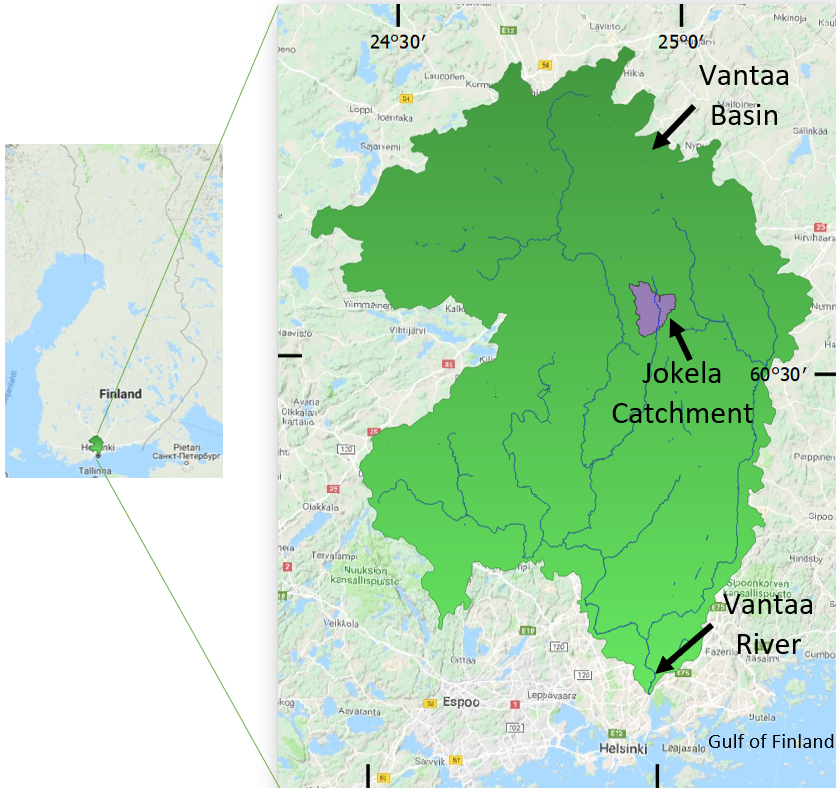
\includegraphics[scale=0.75]{figures/vantaa_basin.png}
	\caption{Vantaa Basin}
	\label{fig:rdiixdwf}
\end{figure}

Jokela is a town located in south region of Finland approximated 40 [km] from the capital city of Helsinki. It is part of Tuusula municipality. Jokela's urban area is mostly residential with an area estimated of 315 [ha]. There are approximated 6500 residents and 2975 buildings (households, commercial, and factories). The area is rather flat with an average slope of 3\%. Its land use can be considered semi-urban and roughly divided as approximated 43\% of its catchment area with forests and semi-natural areas, 32\% with urban artificial surfaces, 13\% of transitional woodland or shrub and 12\% or pastures. Its soil superficial deposit is mostly clay (66\%) and sand (20\%). Its main drainage stream has an rough average of 6.5 [m] width and cuts the catchment flowing from north to south draining to Vataanjoki (Vantaa River) and traveling approximated 50km before reaching the Gulf of Finland. 


\section{Data and Parameter Estimation}

This section presents the details of parameter estimation for the physically-based model (SWMM modules) and RTK-Unit Hydrographs and the data sets used for model construction, calibration and validation. 


%===============================================================
% Sanitary Sewer Inflow Data
%===============================================================

\subsection{Sanitary Sewer Flow Data} \label{flowdata}
    
Flow meter data was provided by Tuusula Water Utility which is responsible for urban drainage system management of Jokela town and all Tuusula municipality. Data was measured at \ac{SSN} pumping stations of which two are used for calibration and validation purposes in this study. One of the meters is located at the last pumping station (Jokela Pumping Station - subcatchment D4S4) of the delineated area and it is considered the system outlet. hourly measurements were recorded during almost whole period of 2018. 
The flow data was pre-processed to eliminate missing data, outliers and normalize it to reduce noisy measurements as an attempt to capture the overall evolution of the flow. Figure x depicts the distribution of measured data before and after the elimination of outliers and missing data. The outliers, flows greater than 200 [l/s], appears as spikes measured only at one data interval unit (1h). This suggests that these measurements are in fact unreal values and were filtered out. Missing measurements were completed using simple linear interpolation. Zero flow measurements were assumed also as missing data. When longer periods of missing data was observed (approximated >12h) were left out of the future analysis: RDII quantity estimation and calibration. 

\begin{figure}[ht]
    \centering
	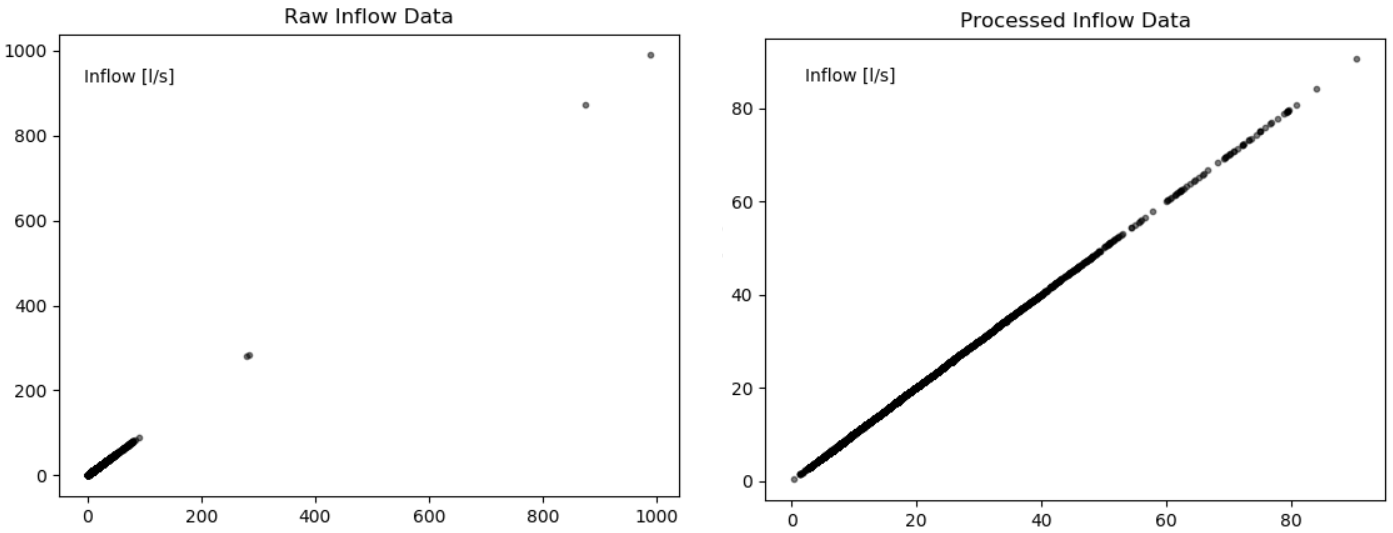
\includegraphics[scale=0.45]{figures/rawinflow_x_processedinflow.png}
	\caption{RDII x DWF estimate for 2018 of total waste water load}
	\label{fig:rdiixdwf}
\end{figure}

Outliers presenting extreme flow were relatively easy to be identified and filtered by defining a threshold and filtering out. However, unreal measurements presenting customary flow rates were harder to be filtered using the threshold method. An example of such measurement is depicted in figure \ref{fig:smoothedflow} on February 22nd at 20:00. The flow data was then smoothed using Savitzky-Golay filter with window length of 11 and 5th order polynomial. It is important to mention that care should be taken when smoothing the data since it can erroneously reduce the peak flow measured. Periods with flows higher than average and peaks are most important when simulating wet-weather flow conditions into \ac{SSN}. Higher order polynomials better reproduce the peak flows, but also keep unrealistic low flows. The pre-treatment procedure is most used for auto-regressive models that use historical flow data not only for comparing the results and calibrating, but also to build the model itselt. \citet{Li2019} performed similar pre-treatment on a sanitary sewer flow data derived from pump ON/OFF operation to transform non-stationary data into stationary before applying autoregressive-moving-average model (ARMAX). 


\begin{figure}[ht]
    \centering
	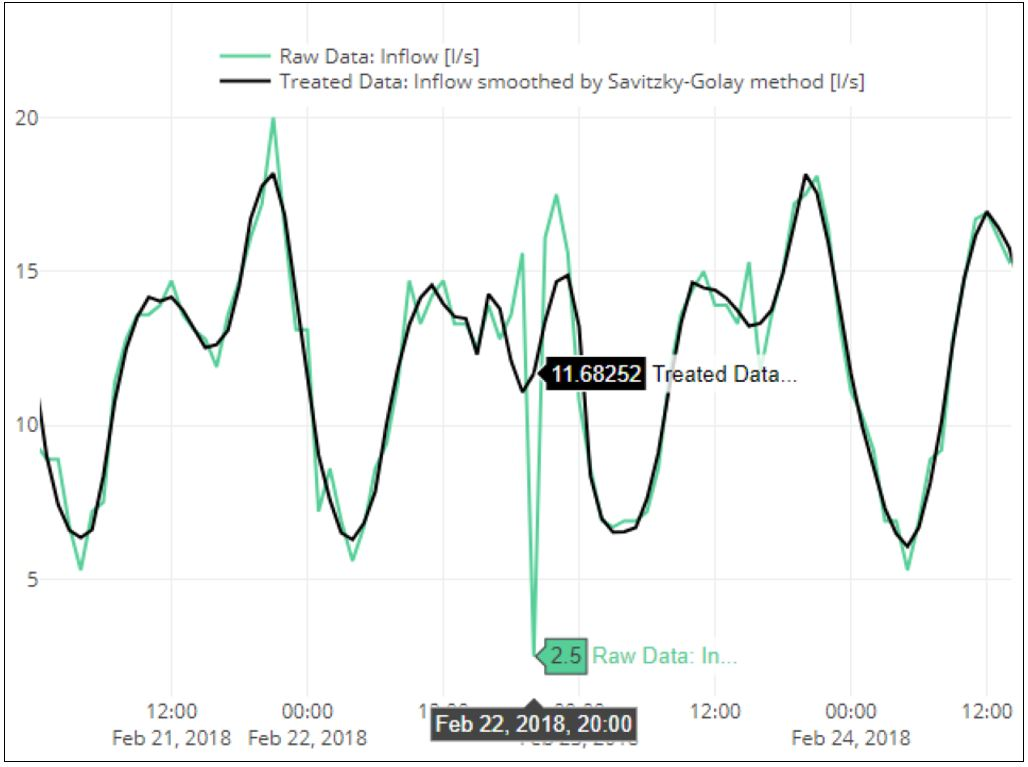
\includegraphics[scale=0.45]{figures/rawinflow_x_processedinflow_smoothed.JPG}
	\caption{RDII x DWF estimate for 2018 of total wastewater load}
	\label{fig:smoothedflow}
\end{figure}

An external script written in python 3 was developed to perform the flow data treatment. Other relevant tool used was the EPA SSOAP toolbox \cite{Vallabhaneni2007}. It helped to identify RDII flows from the raw flow data as described in the following section.
    


\subsubsection{Separation of Sanitary Sewer Flow Components}

It was relevant to identify the different components of the \acf{SSN} to estimate the amount of RDII flows and compare measured with modelled when analysing the water balance for short or long-term simulations. The estimated "measured" RDII flows were identified using EPA SSOAP toolbox.

EPA SSOAP toolbox has many functionaries. As its core, it allows the users to visually build RTK Unit Hydrographs throguh an interative process by adjusting RTK parameters and comparing the output hydrograph with the hydrograph measured \cite{Vallabhaneni2007}. However, the SSOAP toolbox was mostly used in this study to identify precipitation events and identigy the flow components in Jokela's \ac{SSN}. RTK parameters were estimated in this study using an optimization algorithm as described in previous sections.

Two input data were used in SSOAP: 1. Sanitary Sewer Flow Data of Jokela Pumping Station. 2. Precipitation data (better described on section \ref{meteodata}. SSOAP utilizes precipitation data to identify wet-periods and define precipitation events. Days without \acf{WWF} are then filtered to define a mean \acf{DWF} hydrograph for weekdays and weekends. Current day and previous two days with any precipitation record were filtered out of the data set for Weekdays and Weekends. Past three to seven days with precipitation amount record higher than 10 [mm] and 15 holidays in Finland were also filtered out of the set. A total of 66 days weekdays and 32 weekends remained from DWF identification process. The output DWF hydrographs are depicted in figure \ref{fig:ssoapdryh}. Weekdays average daily DWF of 11.4 [l/s] with standard deviation of 1.75 and 12.5 [l/s] and standard deviation of 2.35 for weekends. 
Refer to \citet{Vallabhaneni2007} for detailed information about the SSOAP toolbox.

\begin{figure}[h]
    \centering
	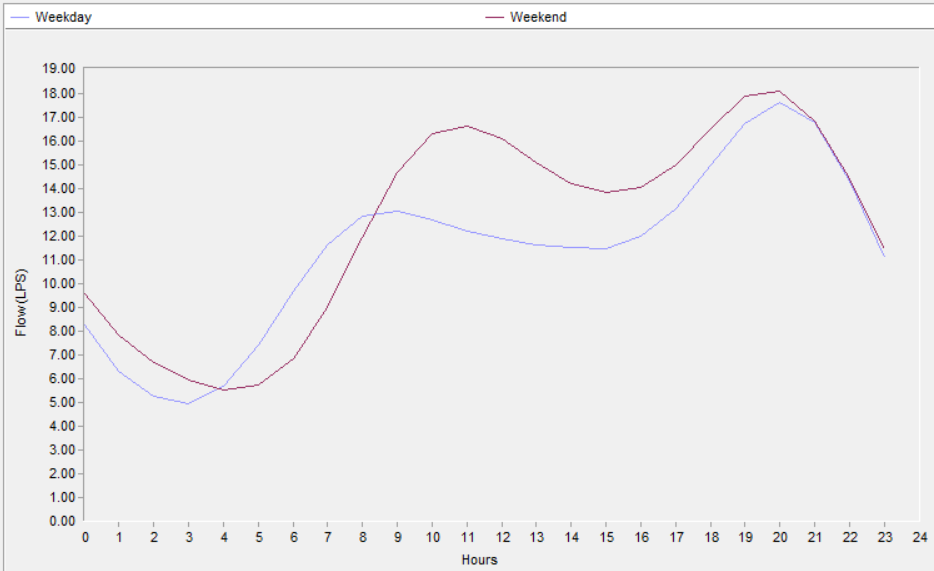
\includegraphics[scale=0.6]{figures/ssoap_dry_hydrograph.png}
	\caption{Estimated Dry-weather Hydrograph from EPA SSOAP tool}
	\label{fig:ssoapdryh}
\end{figure}



The next steps using SSOAP tool were towards subtracting the DWF estimated from metered flow to quantify RDII flow ($RDII = Metered Flow - DWF$). The first step is to define the constant groundwater infiltration (GWI). This is important to further divide the DWF into two parts: Basewaste flow (BWF) and GWI. The GWI is estimated as a percentage of the minimum nighttime flow. SSOAP help file suggest that in residential areas typically 90\% of the minimum nighttime flow represents GWI.However, a different approach was chosen based on available information from the water utility. It was known that an estimate of 900[m³/day] is pumped to Jokela area from the water distribution system. Then, It was assumed that almost all water supplied eventually finds its way to the sanitary sewer network, meaning that the daily average BWF is roughly 900[m³/day]. To achieve this value for BWF with 2018 recorded flow an estimate of 25\% of daily minimum nighttime flows was attributed to GWI with the rest (75\%) representing wastewater flow. Table \ref{tbl:RDIIestimate} depicts the estimated daily average flow components of Jokela's \ac{SSN} with approximated 37\% of the total wastewater amount transported to the \ac{WWTP} being non revenue water (NRW) from RDII and constant GWI. Figure \ref{fig:rdiixdwf} has the monthly amount of the amount of RDII versus DWF with approximated 87\% of total annual RDII amount happening from January to May of 2018.

\begin{figure}[h]
    \centering
	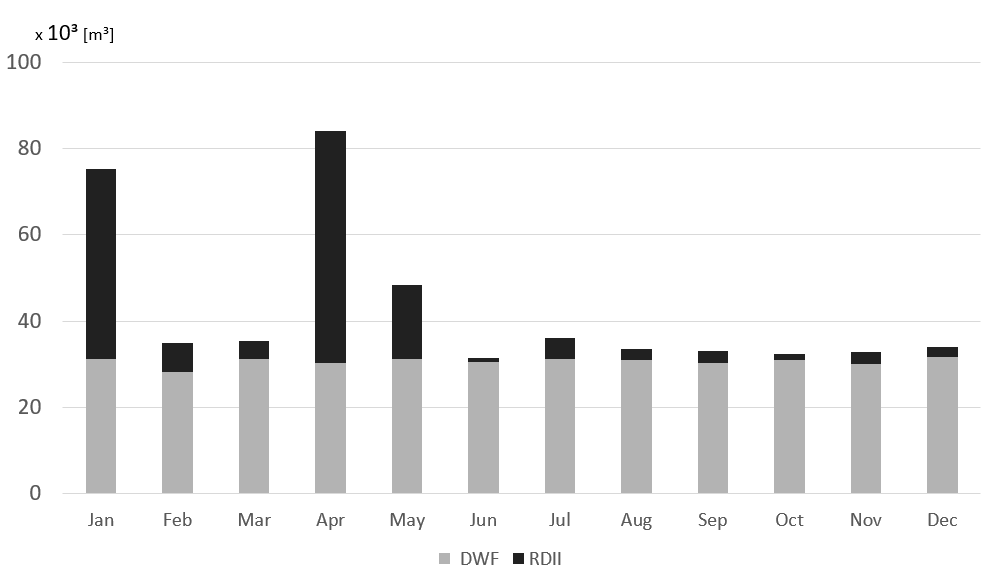
\includegraphics[scale=0.75]{figures/rdii_x_dwf_2018.png}
	\caption{RDII x DWF estimate for 2018 of total wastewater load of Jokela \ac{SSN}}
	\label{fig:rdiixdwf}
\end{figure}


\begin{table}[ht]
\caption{Monthly estimated amount of \acf{SSN} flow components in 2018 for Jokela Catchment in [m³]}
\label{tbl:RDIIestimate}
\centering
\begin{tabular}{cccccccc}
\toprule
\textbf{Month} & \textbf{Obs Flow} & \textbf{DWF}   & \textbf{BWF}   & \textbf{RDII} & \textbf{RDII + GWI} & \textbf{\% RDII} & \textbf{\% RDII + GWI} \\ \hline
Jan            & 2429              & 1007           & 897            & 1423          & 1533                & 58.57            & 63.09                  \\
Feb            & 1241              & 1006           & 896            & 237           & 347                 & 19.13            & 28.00                  \\
Mar            & 1136              & 1010           & 899            & 136           & 246                 & 11.93            & 21.68                  \\
Apr            & 2801              & 1011           & 901            & 1790          & 1900                & 63.90            & 67.85                  \\
May            & 1556              & 1010           & 900            & 547           & 657                 & 35.13            & 42.22                  \\
Jun            & 929               & 1015           & 903            & 32            & 143                 & 3.42             & 15.40                  \\
Jul            & 1041              & 1007           & 897            & 159           & 269                 & 15.33            & 25.89                  \\
Aug            & 932               & 1003           & 894            & 82            & 192                 & 8.80             & 20.58                  \\
Sep            & 1028              & 1011           & 901            & 94            & 204                 & 9.10             & 19.85                  \\
Oct            & 986               & 1003           & 894            & 39            & 149                 & 3.96             & 15.07                  \\
Nov            & 1066              & 1004           & 894            & 89            & 199                 & 8.31             & 18.63                  \\
Dec            & 1025              & 1022           & 910            & 77            & 189                 & 7.51             & 18.45                  \\ \hline
\textbf{Total} & \textbf{16169}    & \textbf{12110} & \textbf{10785} & \textbf{4704} & \textbf{6028}       & \textbf{29.1}    & \textbf{37.3}   \\ \bottomrule      
\end{tabular}
\end{table}

It is import to remember that the RDII flow can also be further divided (i.e. short term hydrograph from runoff and long term hydrograph from subsurface infiltration) and the varying groundwater infiltration happening after rainfall or snowmelt is considered here different than the constant GWI used in SSOAP toolbox. Different GWI in \ac{SSN} were discussed in section \ref{methods_rdii}. 



% Dry Weather Flow Statistics for Meter Flow-Jokela-Smoothed

% Flows are in LPS

%           Average Maximum   Average   Average Minimum
% Weekday       17.5046       11.3026        4.9083
% Weekend       18.0745       12.5058        5.5565



% average Minimum night flow

% 1   15.8.2018   3.0556 LPS
% 2   11.8.2018   3.0556 LPS
% 3   12.8.2018   3.2639 LPS
% 4   18.8.2018   3.3333 LPS
% 5   8.9.2018   3.3333 LPS
% 6   7.8.2018   3.3333 LPS
% 7   20.8.2018   3.4028 LPS
% 8   17.8.2018   3.4028 LPS
% 9   9.9.2018   3.5417 LPS
% 10   8.8.2018   3.6111 LPS




    
    
% WET WEATHER determ
% - minimum peak I/I LPS 0 
% - minimum event duration 6h
% - minimum rainfall volume mm 15


% 9 events defined

% % Event #        Start Date           End Date
% % --------------------------------------------
% % 1          1.1.2018 0.00    1.21.2018 22.00
% % 2        1.21.2018 23.00    2.18.2018 22.00
% % 3         4.9.2018 20.00     5.26.2018 3.00
% % 4        6.21.2018 21.00    6.22.2018 16.00
% % 5          7.3.2018 0.00     7.4.2018 18.00
% % 6         7.4.2018 19.00     7.7.2018 10.00
% % 7        8.20.2018 18.00    8.21.2018 14.00
% % 8        9.11.2018 18.00     9.14.2018 0.00
% % 9         9.15.2018 8.00    9.19.2018 23.00



% - holidays in Finland were not counted (total of 15 days)
% - dry days with no rainfall with a period of X
% - Current, previous and two days previous maximum allowed rainfall amount set to zero. From three to seven previous days maximum rainfall set to 10mm.
% Determining Weekday Statistics...
%  Number of days written = 78
%  Number of days lost    = 286
%                       AVERAGE (LPS)   STANDARD DEVIATION (LPS)
% Average Daily Flow      12.3646                  4.1401
% Maximum Daily Flow      18.6477                  5.3117
% Minimum Daily Flow      6.0559                  3.9778

% Eliminating Weekdays...
%  Number of days written = 66
%  Number of days lost    = 298
%                       AVERAGE (LPS)   STANDARD DEVIATION (LPS)
% Average Daily Flow      11.3778                  1.7468
% Maximum Daily Flow      17.6507                  2.4096
% Minimum Daily Flow      4.9255                  1.5036


% Determining Weekend Statistics...
%  Number of days written = 36
%  Number of days lost    = 328
%                       AVERAGE (LPS)   STANDARD DEVIATION (LPS)
% Average Daily Flow      14.3232                  6.2980
% Maximum Daily Flow      20.5264                  7.9425
% Minimum Daily Flow      7.0682                  5.5326

% Eliminating Weekend days...
%  Number of days written = 32
%  Number of days lost    = 332
%                       AVERAGE (LPS)   STANDARD DEVIATION (LPS)
% Average Daily Flow      12.5058                  2.3451
% Maximum Daily Flow      18.3138                  2.9730
% Minimum Daily Flow      5.4570                  2.2070


% - \& of GWI assumed
% -there were X available days after excluding the above mentioned. The mean flow for each hour of these days was defined as the DWF.


% Include Table here with "water balance" 
% - Month - Peak Flow [l/s] - Mean flow [l/s] - NRW [m³] - \% of GWI


% Before smoothing
% Maximum Flow = 90.600 LPS @ 5.7.2018 1.00.00
% Minimum Flow = 0.300 LPS @ 4.6.2018 12.00.00
% Average Flow = 15.104 LPS

% after smoothing
% Maximum Flow = 81.573 LPS @ 5.1.2018 10.00.00
% Minimum Flow = 1.701 LPS @ 12.8.2018 4.00.00
% Average Flow = 15.104 LPS





%===============================================================
% Meteorological data
%===============================================================

\subsection{Meteorological Data \& Parameters} \label{meteodata}

Meteorological data is presented for both historical and weather forecast. The first is used in this study as input for hydraulic models during calibration and validation process whereas the forecast is utilized to compare the model performances using HARMONIE model forecast. Precipitation data is used for both physically-based and RTK unit hydrograph method. Snow depth measurements were used as input for the snowpack \& snowmelt SWMM module process and to calibrate its parameters.


%   Precipitation data
    
\subsubsection{Precipitation}
[TO DO]\\ \\
- Relevant characteristics of precipitation data (monthly amount, intense precipitations, snowfall and rainfall, etc)\\
- maybe further comparison of 2018 precip. data and past 10 years.\\
- possible data treatment (i.e. missing values)\\
- rain gauge used\\
- how precip. data was input to the models\\
- Events chosen for calibration.\\


%   Temperature data

\subsubsection{Temperature}

[TO DO]\\ \\
- Relevant characteristics of Temp. data \\
- maybe further comparison of 2018 Temp. data and past 10 years.\\
- possible data treatment (i.e. missing values)\\
- how temp. data was input to the models\\


Note: One missing data that was filled using linear interpolation between the previous and next hour.

%   Wind data

\subsubsection{Wind}
[TO DO]\\ \\
- Relevant characteristics of wind data (average speed and direction) \\
- maybe further comparison of wind data from different weather stations \\
- possible data treatment (i.e. missing values)\\
- how wind data was input to the models\\


%   Snow data and param estimation

\subsubsection{Snow Depth \& Snowpack Parameters}

[TO DO] \\

-brief comments on the snowdepth data (measure method, location of the measurements and the limitation when extrapolating for the entire catchment area \\ \\ \\

\begin{figure}[h]
    \centering
	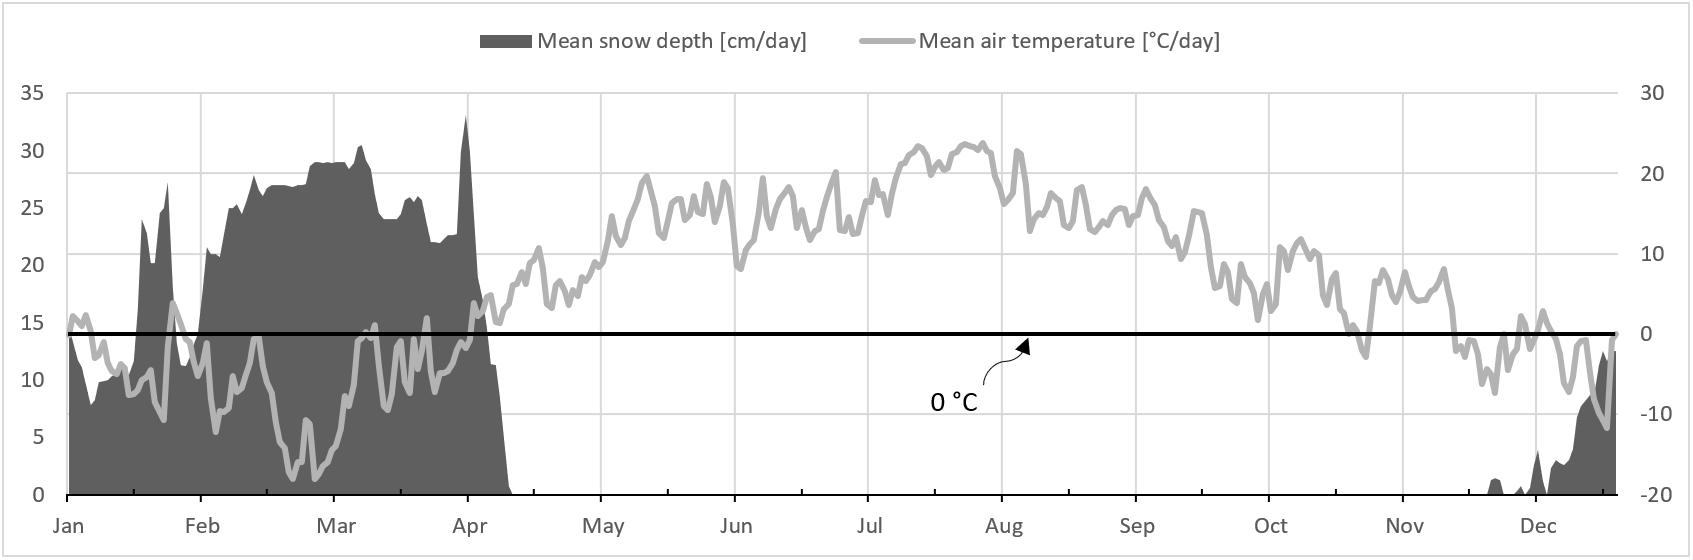
\includegraphics[scale=0.45]{figures/measuredsnowpack.png}
	\caption{Snow depth and Temperature Measurements \citet{fmidata}}
	\label{fig:snowmeasurement}
\end{figure}
        
Estimation of parameters was carried based on the range proposed in section \ref{snowlit}. Sensitivity analysis was carried by manually varying individual parameters while others were static. It was found that the degree-hour melt coefficients ($DHM_{min}$, $DHM_{max}$), dividing temperature ($SNOTMP$), base temperature ($T_{base}$) and snow catch factor ($SCF$).

Base temperature and dividing temperature were initially estimated by observing relations among hourly temperature and snow depth. Whenever the snow depth measurement varied, values of temperature where collected. Temperatures during the increase of the snow depth were stored to estimate the dividing temperature($SNOTMP$) whereas temperatures during decrease of snow depth were used to estimate the base temperature($T_{base}$). Periods when the temperatures were out of the range limited (see table \ref{tbl:snowparam}) were discarded. The mean of the stored temperature were then used as the final estimation of $SNOTMP$ and $T_{base}$ and were respectively  0.1°C and -1.9°C. It is important to emphasize that this was a rough estimate used only to input initial values for the simulations. $DHM_{min}$ and $DHM_{max}$ were set initially as the limits of table \ref{tbl:snowparam}. $TIPM$ and $RNM$ were set as used by \citet{Rossman2016} and \citet{anderson1973}. No information on the rain gauge deficiency to record snowfall and fraction of free water capacity values were assessed. Therefore, $SCF$ and $FWFRAC$ values were set initially to their middle range. Two parameters for initial condition of the simulation are also required: 1. Initial depth of water equivalent ($SD_0$); 2. initial free water ($FW_0$). The first was estimated as 10\% of the first measured value of snow depth assuming a ratio of 10:1 for the snow pack depth and water equivalent depth as rule of thumb suggested by \citet{Rossman2016}.
    
Figure \ref{fig:snow1sim} show the results of the simulation using the initially estimated parameters and the results of a simulation with parameters manually calibrated. Four first months of 2018 between 1\textsuperscript{st} of January and 15\textsuperscript{th} of April when all the snow depth measured was already melted.

\begin{figure}[h]
    \centering
	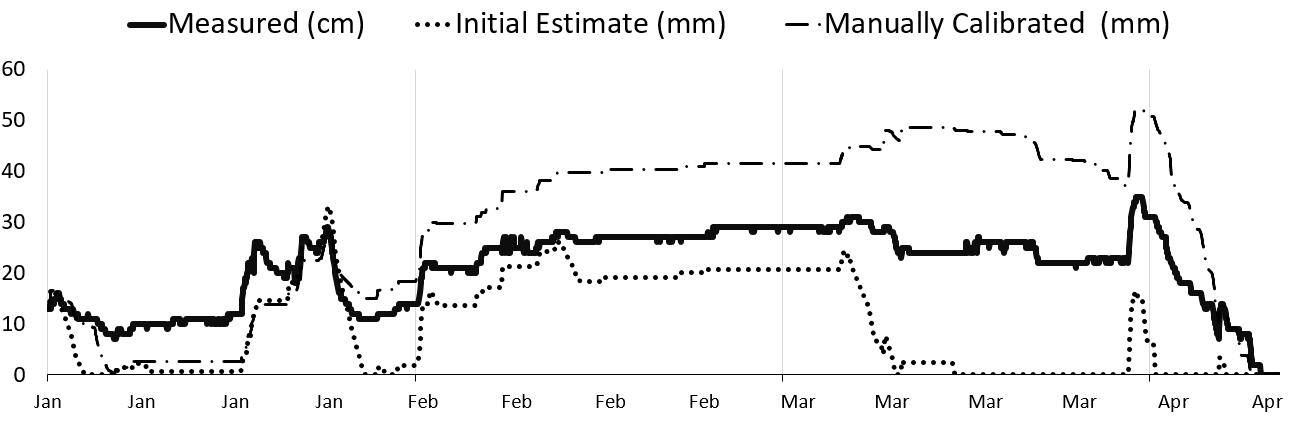
\includegraphics[scale=0.55]{figures/snowdepth_1st_simulations.png}
	\caption{Results of Initial parameter estimation x manual calibration of Snowpack \& Snowmelt parameters}
	\label{fig:snow1sim}
\end{figure}
    
By a visual analysis of the results of the first simulation and comparison to the measured snow depth values, it is possible to identify a higher rate of melt and snow accumulation than the values measured. This was corrected after a manual calibration of parameters. A lower rate of snow accumulation was achieved by assuming that the rain gauge was able better measure the snowfall. Therefore, $SCF$ was reduced to 1.2. To reduce melting rate, the temperature which snow melt starts ($T_{base}$) was increased to its upper limit of 0°C. Although the results were better, a higher melt rate than expected was still with the pack being completely melted around three weeks before the expected time. Therefore, the minimum melt coefficient ($DHM_{min}$) was lowered further than its lower range limit from 0.019[mm/°C-h] to 0.001[mm/°C-h].

%SCF, among the sensitive parameters, were calibrated aiming to find a smaller range of sensitive parameters to describe the study area reducing the amount of possible values. 

Table \ref{tbl:snowparamest} depicts the initially estimated parameters, parameter values after manual calibration against measured data, and changes in the previously proposed range based on literature review (see table \ref{tbl:snowparam}) after results of the manual calibration. The only changed was a reduction of $DHM_{min}$ parameter of approximated 47\%. 

\begin{table}[h]
\caption{Snowpack \& Snowmelt estimated parameters \cite{Rossman2016}}
\label{tbl:snowparamest}
\centering
\begin{tabular}{lcccc}
\toprule
\textbf{Parameter} & \textbf{\begin{tabular}[c]{@{}c@{}}Initially\\ Estimated\end{tabular}} & \textbf{\begin{tabular}[c]{@{}c@{}}Manually\\ Calibrated\end{tabular}} & \textbf{\begin{tabular}[c]{@{}c@{}}Changes in \\ Previous Range\end{tabular}} & \textbf{Calibrated} \\ \hline
SNOTMP             & 0.1                                                                                        & 0.1                                                                                        & -                                                                                                 & {[}°C{]}            \\
SCF                & 1.5                                                                                        & 1.2                                                                                        & -                                                                                                 & {[}1{]}             \\
T\textsubscript{b}                 & - 1.9                                                                                      & 0                                                                                          & -                                                                                                 & {[}°C{]}            \\
DHM\textsubscript{min} - DHM\textsubscript{max}          & 0.019 - 0.10                                                                               & 0.009-0.03                                                                                 & 0.009 - 0.15                                                                                      & {[}mm/°C-h{]}       \\
RNM                & 0.6                                                                                        & 0.6                                                                                        & -                                                                                                 & {[}1{]}             \\
FWFRAC             & 0.13                                                                                       & 0.13                                                                                       & -                                                                                                 & {[}1{]}             \\
TIPM               & 0.5                                                                                        & 0.5                                                                                        & -                                                                                                 & {[}1{]}             \\
SD\textsubscript{0}                & 13                                                                                         & 13                                                                                         & -                                                                                                 & {[}mm{]}            \\
FW\textsubscript{0}                & 0                                                                                          & 0                                                                                          & -                                                                                                 & {[}mm{]}           
\\ \bottomrule
\end{tabular}
\end{table}


% Forecs werelocati calconast data
\subsection{Weather Forecast}
[To Do]\\\\

- Description of Harmonie weather forecast data provided from FMI\\
- grid resolution of 2.5km, Weather forecast variables and rainfall up to h+ 66h, forecast Updated every 6 hours, lambert's projection\\
- Description of the routine created for automatic data acquisition from FMI APIs\\

\begin{figure}[ht]
    \centering
	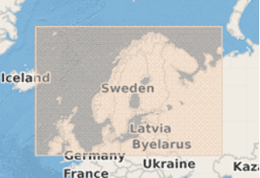
\includegraphics[scale=1.2]{figures/harmoniecoverage.png}
	\caption{HARMONIE weather model forecast coverage}
	\label{fig:harmonie}
\end{figure}



%===============================================================
%   Topographic data
%===============================================================
        

\subsection{Topographic Data \& Parameters}

Topographic data was assessed to estimate parameters used to model different flows happening in Jokela's catchment. The chart presented in figure \ref{fig:topoxprocess} shows the relation among topographic data sets and the process being modeled. 

\begin{figure}[h]
    \centering
	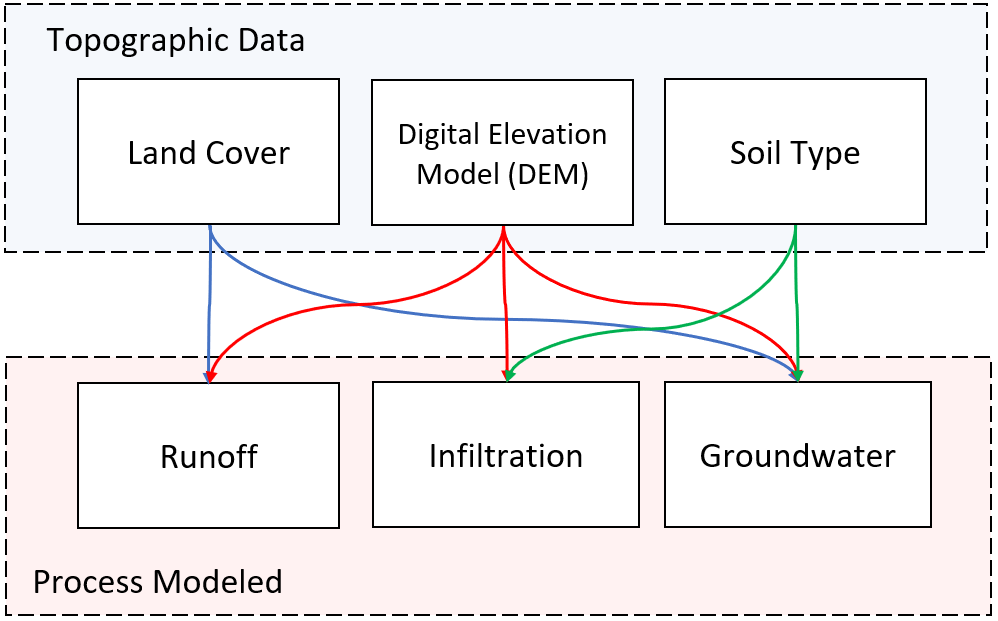
\includegraphics[scale=0.5]{figures/topo_x_process.png}
	\caption{Topographic data used per each Modeled Process}
	\label{fig:topoxprocess}
\end{figure}

Data description and initial parameter estimates are provided in the following sections. 

% Runoff parameters
\subsubsection{Terrain Data \& Runoff Parameters} \label{runoffcs}
    
The Digital Elevation Model (DEM) was used in many parts of this study. It is used in the Runoff model to delineate the subcatchments that provided area information for all the SWMM modules used. The DEM used is this study was provided by the National Land Survey of Finland (NLS) through its open data platform as 2 x 2 [m] resolution based on laser scanning data collected in the summer of 2015. The vertical resolution varies from 0.3 to 1 meter \cite{nsldata}. The DEM provided had already bridges cut off and a "filling" operation was caried using Qgis to exclude possible holes existent in the data set.

The definition of the \texttt{\textit{Area}} parameter for \acf{SSN} is rather conceptually challenging since the pipe network is located under the surface. As mentioned previously, surface and groundwater flow influence \ac{SSN} and their delimited area (watershed or aquifer) as distinct. This can be imagine with the classical example of a rain drop falling over a specific point on the soil surface. The drop can flow over the surface towards the direction of the steeper slope or infiltrate and then flow through the porous in the soil to very different direction than it would flow if remained on the surface. Boundaries of a catch basin can be defined using the highest elevations such as topographic crest and road center line or lowest points of the area such as rivers and streams \cite{Lee2017}. Cadastral parcels, which are property developed urban areas, are also often used to delineate the sewer catch basin. However, parcels are rather divided for administrative reasons than soil or subsoil characteristics. Thus, it can be challenging to estimate some topographical parameters such as soil surface slope and roughness using administrative areas. As a hypothetical exercise one can imagine the possible issue when using parcels when modelling a urban area surrounded by mountains. In case the delineated area is limited only to the properties, no information relative to the mountains' is included in the parameter estimation and simulated hydrographs can mismatch the observed by volume and shape.

The sewershed delineation is, therefore, a discretization of the space domain. In this study, it is assumed as the area division that supplies water to a specific point within the \ac{SSN}. The DEM is usually the data assessed to delineate the area of influence when modeling natural rivers. This method, however, is not conceptually valid for \ac{SSN} once the network's slopes are not always follows the soil surface slopes estimated with the DEM. Therefore, \ac{SSN} has a different slope gradient than the soil surface in some parts and pumping stations are required to transport waste water towards the \acf{WWTP}. This is one of the reason why the space domain was discretized per pumping station in this study. The second reason is that flow meter observations was available for two pumping stations within the catchment and the remaining stations are probably the best candidates to receive flow meter devices in the future. 

DEM, pumping station locations and pipe network were the data used for the subcatchments delineation. Qgis application was chosen to perform GIS operations and delineate sewersheds due to its free open services and embedded automatic delineation tools such as $GRASS - r.watershed$. Proposed subcatchment partition for Jokela town is depicted in figure \ref{fig:subcatchments}

\begin{figure}[h]
    \centering
	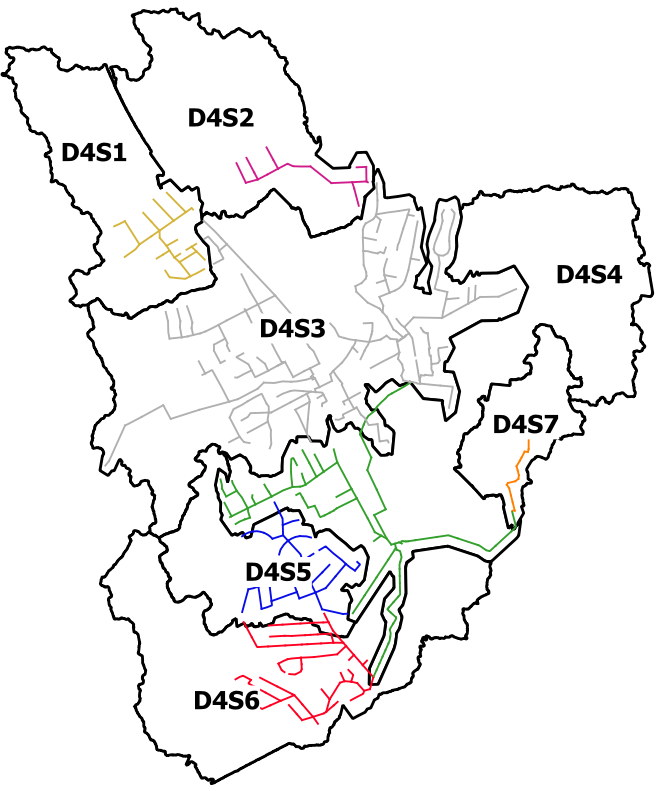
\includegraphics[scale=0.6]{figures/subcatchments.png}
	\caption{Jokela Subcatchment division}
	\label{fig:subcatchments}
\end{figure}



Pumping stations are usually located in areas with lower surface elevation when compared to its upstream pipe network to direct the flow utilizing gravitational force and reduce energy consumption. However, differences between soil surface and network still exists in some parts of the pumping station upstream service area. This happens because no information about soil type and infiltration rates is used when delineating the areas. Therefore, subcatchment of pumping station one (PS 1) may overlay the pipe network upstream pumping station (PS 2). Only automatic sewershed delineation procedure and DEM is not enough to avoid overlaying. To overcome this, a pipe network buffer area can be delineated and summed with its subcatchment or the pipe network vector data can be "burned" into the DEM raster data. Figure \ref{fig:filledxburned} depicts the differences on watershed delineation using $GRASS - r.watershed$ and a "Filled DEM" vs. "Burned DEM".

\begin{figure}[h]
    \centering
	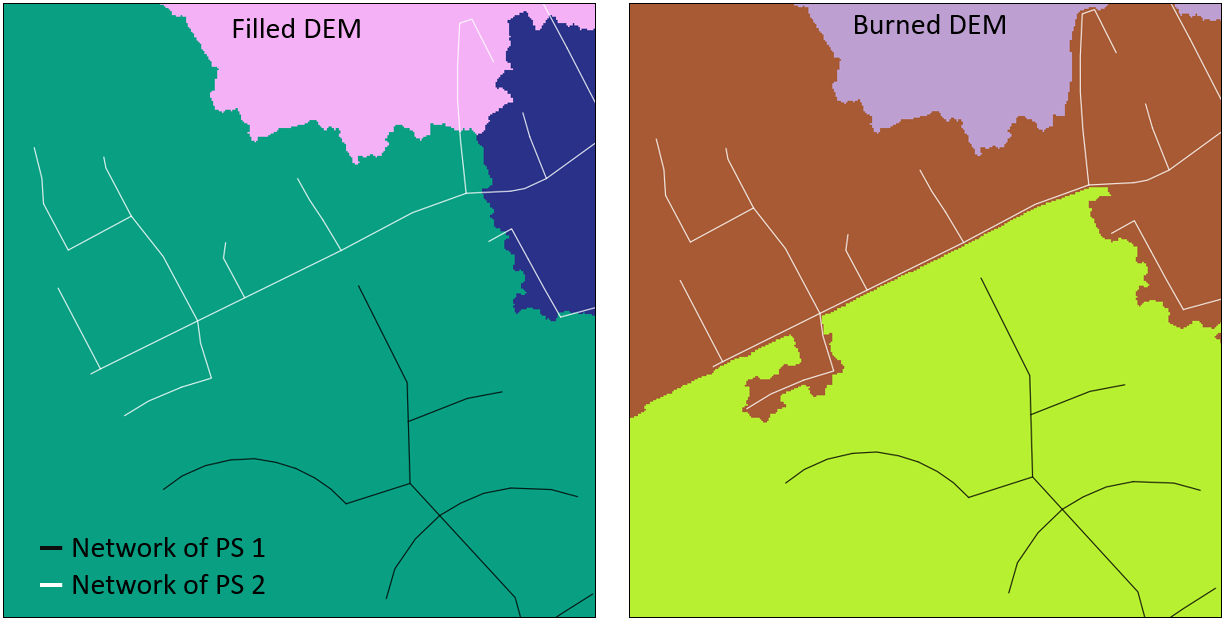
\includegraphics[scale=0.6]{figures/burnedxfilledDEM.png}
	\caption{Comparison of sewershed delineation using Filled and Burned DEM}
	\label{fig:filledxburned}
\end{figure}


The pipe network included in the DEM acts as an artificial stream and successfully limits the subcatchment to its pumping station when pipes from different pumping station do not cross. Some level of manual adjustment is still required when pipe crossing exists.
Other possible way to delineate the area influencing RDII flows into \ac{SSN} is to assume that the area of influence is proportional to the size of the network components (i.e. pipe length and diameter). This assumes that the amount of defect (i.e. pipe cracks) increases when the size of the pipe also increases. In this study a combination of the buffer area proportional to the pipe length and diameter and the topographic crest was used to delineate the subcatchments depicted in figure \ref{fig:subcatchments}. Further adjustments could still be done considering roads, railways, artificial barrers and streams present in the study area. Figure \ref{fig:d1d3} depicts the two different delineation methods (D1 = buffer over pipe size, D3 = topographic crest delineation) used for the final delineation (D4 = D1 + D3).

\begin{figure}[h]
    \centering
	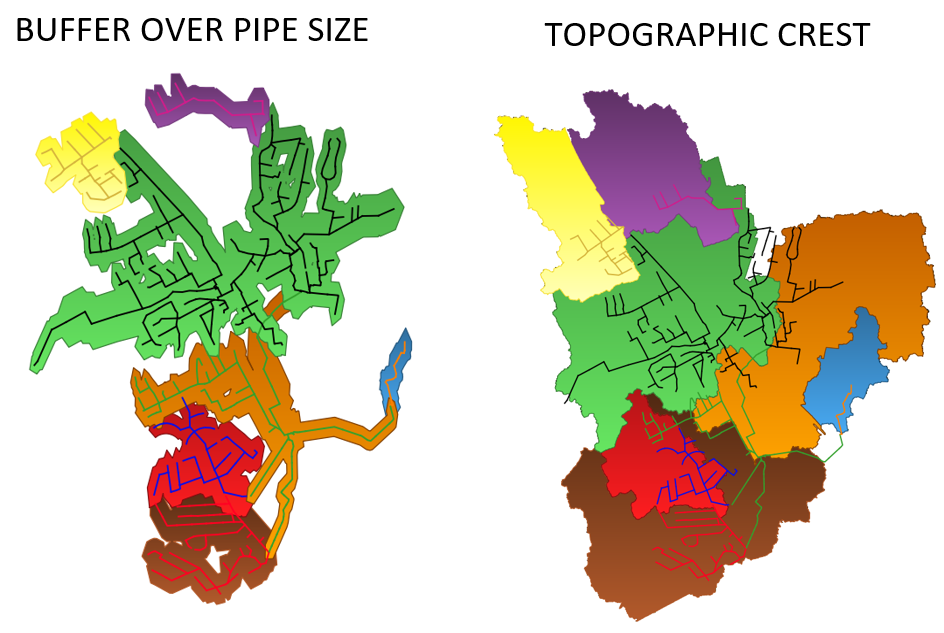
\includegraphics[scale=0.6]{figures/d1_plus_d3.png}
	\caption{Delineation methods D1 (left) and D3 (right)}
	\label{fig:d1d3}
\end{figure}

For organizational purposes, subcatchments where named after delineation method (i.e. D4) and subcatchment id number (i.e. S2). For simplicity the letter were droped and they are reffered hereafter simply by the numbers (i.e. 42). 
call the table and talk about the outlet (D4S4)
INCLUDE Table with the area of each subc, network size, subcatchment area/total area, Subcatchment Area/Pipe Length, and totals.
    
To define other parameters used in SWMM's runoff module a Land Cover data set was assessed. The $Finnish Corine Land Cover 2018$ (CLC2018) distributed by SYKE's open data platform. This data is an essemble of different datasets such as Topographic database, digital road database of finland, building, land parcels and also data interpreted data from satellite images. The source data are from 2016-2017 period and the final raster data has 20m resolution. This dataset was produce by SYKE as part of EU Copernicus Land project and follows its standard nomenclature for land cover class. The raster dataset has four hierarchy levels of land cover class and several sub-classes \cite{sykedata}. If all four hierarchy levels and their sub-classes are used, a better spatial representation of land cover is obtained. However, the choice of which level to use depends on the size of the delineated sewershed. For this study three level of hierarchy were assumed to suffice. The vectorized and clipped dataset for the study area is depicted in figure \ref{fig:landcover}. 


\begin{figure}[h]
    \centering
	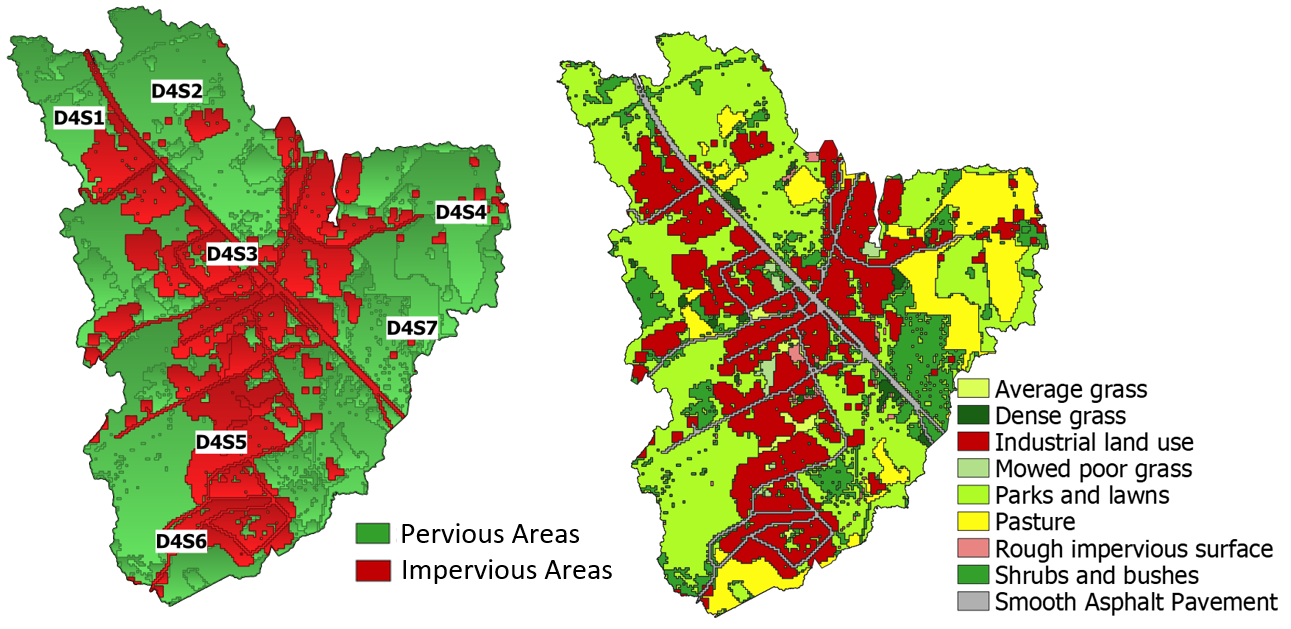
\includegraphics[scale=0.6]{figures/land_cover.png}
	\caption{Pervious and Impervious division (left) and level 3 from SYKE's corine land cover for Jokela catchment (right) \cite{sykedata}}
	\label{fig:landcover}
\end{figure}

Land cover of artificial surfaces were assumed as impervious areas whereas agricultural, forest, seminatural and wetlands assumed as pervious areas.This division was then used to calculate the percentage of impervious area, an input parameter for SWMM runoff module. The roughness coefficient (n manning's) was estimated also from the land cover. For this, a relation between standard copernicus land cover class description and manning's roughness coefficient table available in the literature (\cite{Rossman2016}) was created. An area weighted average calculation was carried as different types of land cover and, therefore, roughness coefficients are present within a subcatchment. In other words, roughness coefficients of land cover with higher percentage over the total subcatchment's area have higher influence in the final value assigned to the subcatchment. This was done for both impervious and pervious area roughness estimate. 
The depression storage parameter were roughtly estimated based on recommendations from Denver Urban Drainage and Flood Control District (UDFCD, 2007). The percentage of impervious land covers areas within a subcatchment were multiplied by 2.54[mm] and pervious land cover areas by 10.16[mm] before the area weighted average was taken. Table \ref{tbl:runoffparamest} depicts the estimated values for runoff parameters for each subcatchment as well as some relations to their respective \ac{SSN}.
    
\begin{table}[h]
\caption{SWMM Runoff parameter estimation}
\label{tbl:runoffparamest}
\centering
\footnotesize	
\begin{tabular}{ccccccccccc}
\toprule
\textbf{sub}                                           & \textbf{\begin{tabular}[c]{@{}c@{}}area \\ {[}ha{]}\end{tabular}} & \textbf{\begin{tabular}[c]{@{}c@{}}area/\\ total\\ {[}\%{]}\end{tabular}} & \textbf{\begin{tabular}[c]{@{}c@{}}Mean\\ Slope \\ {[}\%{]}\end{tabular}} & \textbf{\begin{tabular}[c]{@{}c@{}}n\_imp\\ {[}s/m\textsuperscript{1/3}{]}\end{tabular}} & \textbf{\begin{tabular}[c]{@{}c@{}}n\_perv\\ {[}s/m\textsuperscript{1/3}{]}\end{tabular}} & \textbf{\begin{tabular}[c]{@{}c@{}}Imp.\\ area \\ {[}\%{]}\end{tabular}} & \textbf{\begin{tabular}[c]{@{}c@{}}Ds imp\\ {[}mm{]}\end{tabular}} & \textbf{\begin{tabular}[c]{@{}c@{}}Ds perv\\ {[}mm{]}\end{tabular}} & \textbf{\begin{tabular}[c]{@{}c@{}}Area/\\ net\\ {[}m{]}\end{tabular}} & \textbf{\begin{tabular}[c]{@{}c@{}}Mean \\ elev{[}m{]}\end{tabular}} \\ \hline
41                                                     & 133.5                  & 9.7                                                                    & 6.33                                                                   & 0.0321                                                              & 0.081                                                                & 34.6                                                                  & 0.88                                                               & 6.64                                                                & 488                                                                        & 87.36                                                                \\
42                                                     & 156.8                  & 11.6                                                                   & 6.05                                                                   & 0.0323                                                              & 0.075                                                                & 10.6                                                                  & 0.27                                                               & 9.08                                                                & 889                                                                        & 80.20                                                                \\
43                                                     & 382.9                  & 28.3                                                                   & 5.90                                                                   & 0.0317                                                              & 0.082                                                                & 52.5                                                                  & 1.33                                                               & 4.83                                                                & 179                                                                        & 77.10                                                                \\
44                                                     & 313.9                  & 23.2                                                                   & 4.89                                                                   & 0.0310                                                              & 0.077                                                                & 25.1                                                                  & 0.64                                                               & 7.61                                                                & 315                                                                        & 71.97                                                                \\
45                                                     & 97.7                   & 7.2                                                                    & 6.05                                                                   & 0.0310                                                              & 0.081                                                                & 49.4                                                                  & 1.25                                                               & 5.14                                                                & 240                                                                        & 77.78                                                                \\
46                                                     & 212.2                  & 15.7                                                                   & 6.01                                                                   & 0.0309                                                              & 0.076                                                                & 29.1                                                                  & 0.74                                                               & 7.20                                                                & 363                                                                        & 73.02                                                                \\
47                                                     & 58.1                   & 4.3                                                                    & 2.61                                                                   & 0.0350                                                              & 0.092                                                                & 1.3                                                                   & 0.03                                                               & 10.03                                                               & 930                                                                        & 71.09                                                                \\ \hline
\begin{tabular}[c]{@{}c@{}}sum* / \\ mean\end{tabular} & 1355*                  & 100*                                                                   & 5.41                                                                   & 0.0323                                                              & 0.0806                                                               & 28.9                                                                  & 0.74                                                               & 7.22                                                                & 486.3                                                                      & 76.93                                                               
\\                                                               \bottomrule
\end{tabular}
\end{table}



% Infiltration Parameters

\subsubsection{Soil Superficial Deposits \& Infiltration Parameters}
\label{infiltrationcs}
    
The soil type coverage data was fetched from \acf{GTK} \cite{gtkdata} through its open data online service and was used to estimate the three parameters of Horton infiltration (see, \ref{infiltration}). The available information was obtained as vector data containing superficial deposits of Finland with material produced between 1972-2007. GIS operations were carried using Qgis to delimit the area concerned Jokela's catchment. Coverage of superficial deposit is depicted in figure \ref{fig:supdeposits}. Mixed soil types were simplified to facilitate model's parameter estimations.\\
    
\begin{figure}[h]
    \centering
	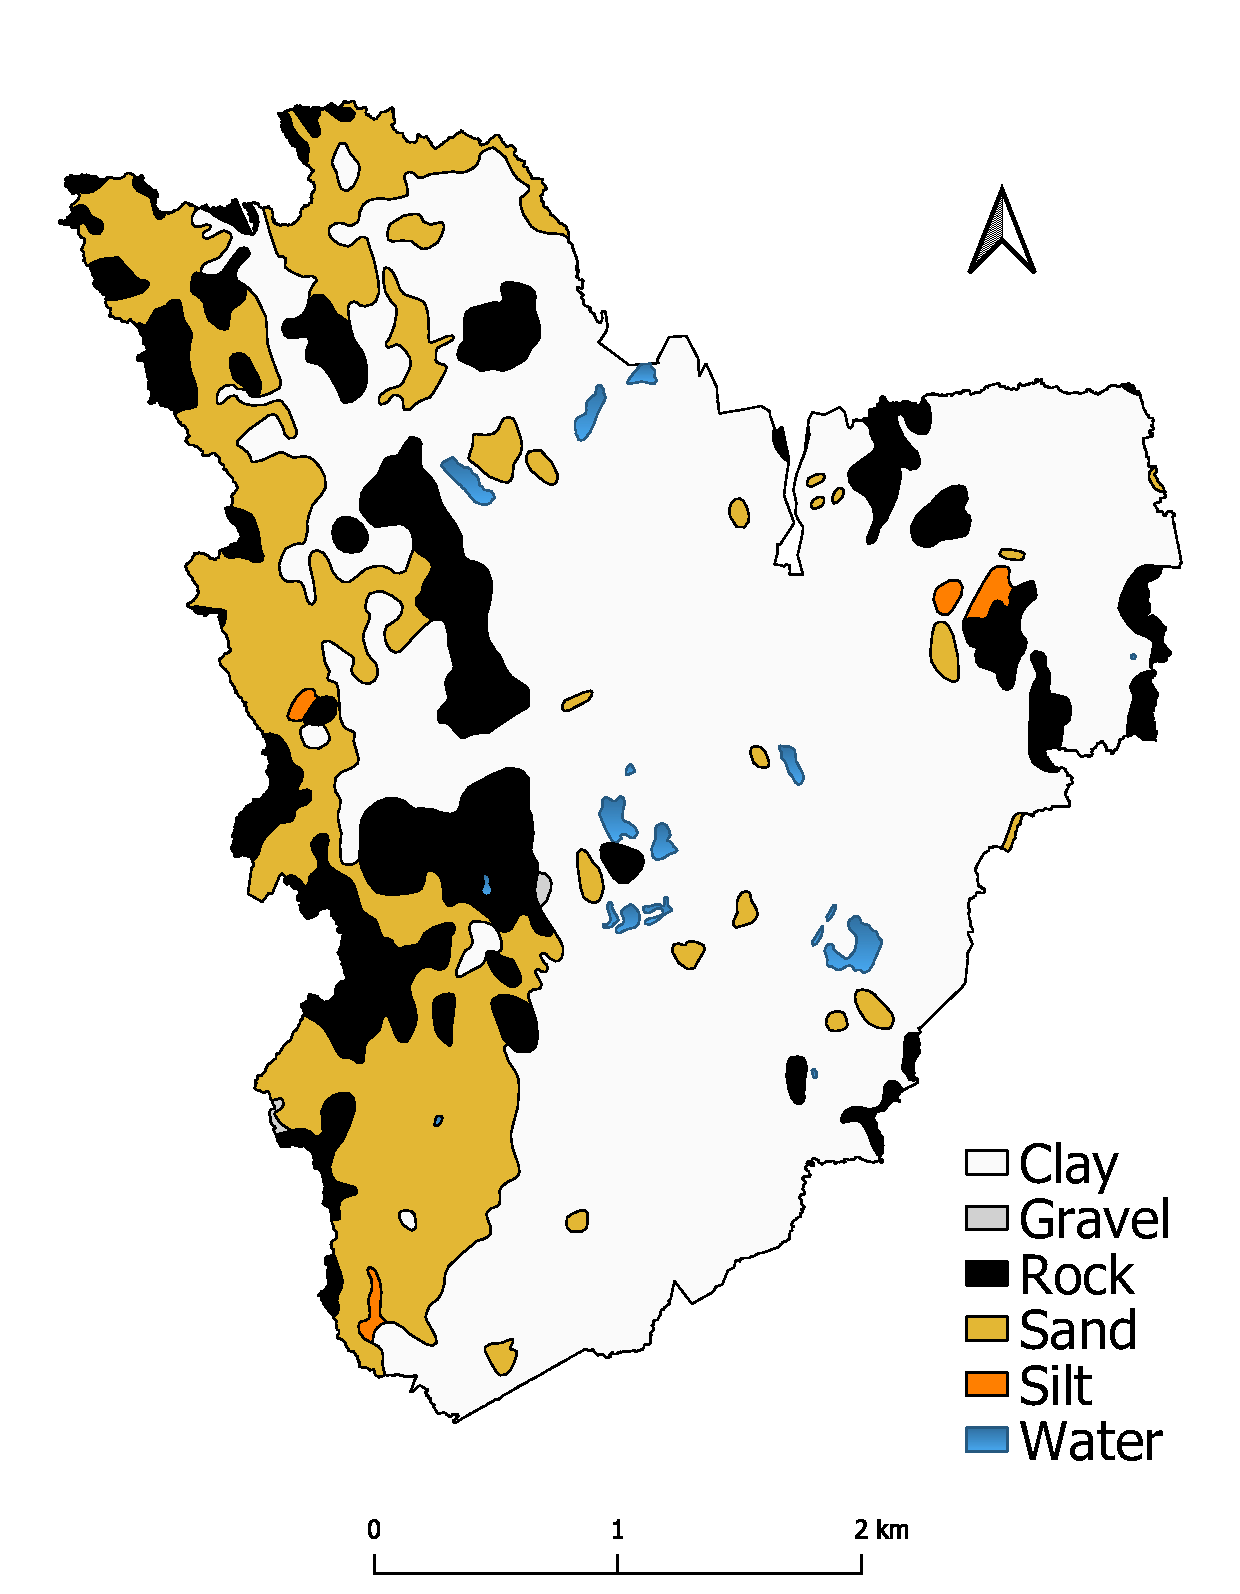
\includegraphics[scale=0.4]{figures/Jokela_Superficial_Deposits.pdf}
	\caption{Jokela catchment soil superficial deposits}
	\label{fig:supdeposits}
\end{figure}

As informed in section \ref{infiltration}, there are four parameters necessary to satisfy the Modified Horton infiltration model: Initial infiltration capacity ($f_0$); Minimum infiltration capacity ($f_\infty$), decay coefficient ($k_d$), and recovery coefficient ($k_r$) that is calculated based on drying time. For simplicity, the parameters were averaged by the whole area of Jokela catchment without considering subcatchment's divisions per pumping station. Therefore, it is assumed that all subcatchments have the same parameters for the infiltration model. Estimation of parameters was carried as follows:
\begin{enumerate}
    \item Initial infiltration capacity ($f_0$): values per soil type as estimated by \citet{Rossman2016} for DRY soils multiplied by 1.2 to account for vegetation present in the catchment.
    \item Minimum infiltration capacity ($f_\infty$): considered equal to saturated hydraulic conductivity with values estimated by \citet{Rawls1983} and available in SWMM user help.
    \item Decay coefficient ($k_d$): set to 4 [h\textsuperscript{-1}] as suggested by \citet{Rossman2016}.
    \item Recovery coefficient ($k_r$) in days: equation \ref{eqn:k_r} as function of minimum infiltration capacity in inches/hour.
\end{enumerate}

\begin{equation}
\label{eqn:k_r}
k_r = \frac{3.125}{\sqrt{f_\infty}}
\end{equation}


The estimation of each parameter for each soil type is depicted in table \ref{tbl:infparamest}. Area and percentage of coverage for each soil type was also calculated to spatially weight $f_0$, $f_\infty$, and $k_r$ using equation \ref{eqn:infilaverage} to obtain a unique value of each parameter to represent the entire catchment.


\begin{table}[h]
\caption{Modified Horton infiltration parameter estimation}
\label{tbl:infparamest}
\centering
\begin{tabular}{@{}lccccc@{}}
\toprule
\textbf{soil type} & \textbf{area [ha]} & \textbf{coverage [\%]} & \textbf{$f_0$} & \textbf{$f_\infty$} & \textbf{$k_r$} \\
\midrule
Clay               & 887.5                 & 66.0                       & 30.5          & 0.3                            & 28.8          \\
Sand               & 267.9                 & 19.9                       & 152.4         & 117.8                          & 1.5           \\
Rock               & 181.6                 & 13.5                       & 3.0           & 0.03                            & 90.9          \\
Silt               & 5.9                   & 0.4                        & 91.4          & 6.5                            & 6.2           \\
Gravel             & 1.2                   & 0.1                        & 1524.0        & 1180.0                         & 0.5           \\
Water              & 11.5                  & 0.9                        & -             & -                              & -             \\ \midrule
Total              & 1355.7                & 100.0                      & -             & -                              & - \\           
\bottomrule
\end{tabular}
\end{table}

\begin{equation}
\label{eqn:infilaverage}
Parameter = \sum_{n}^{m}(Parameter_n \cdot Coverage_n \cdot 0.1)
\end{equation}
where: \\
\indent $parameter$ = $f_0$, $f_\infty$ or $k_r$ \\
\indent $n$ = soil type (excluding water) \\

after applying equation \ref{eqn:infilaverage} was applied to the estimated parameters of table \ref{tbl:infparamest}. The result of $k_r$ was set to its upper limit range since it was greater than 14 days because of the predominance of soil types with relatively low saturated hydraulic conductivity (\textit{Clay and Rock}). The following unique parameters were obtained and included to SWMM model:

\begin{center}
  $f_0$ = 52.2 [mm/h], $f_\infty$ = 24.6 [mm/h], $k_d$ = 4 [1/h], $k_r$ = 14 [days]  
\end{center}





%===============================================================
%   Groundwater Data and Groundwater Flow Parameters
%===============================================================

\subsection{Water Table \& Groundwater Flow Parameters} \label{gwcs}

As mentioned in the literature \citet{Bennett1999,Vallabhaneni2007,Barden2015}, infiltration into the sewer lines can be caused by the seasonal elevation of groundwater table or other condition that increased soil moisture content causing a temporary saturated zone. Elevation of the groundwater table around Jokela town was assessed in this section as an attempt to identify a possible correlation with seasonal variations of the water table and the flow measurements of the town’s sanitary sewer network. 
Information of water table levels was collected from the Finnish Environmental Institute (SYKE) through its open data service \cite{sykedata} and provided by Tuusula Water Utility. Data of three observation wells from SYKE were available surrounding and Jokela town and one from Tuusula Water Utility database within the delineated catchment as depicted in figure \ref{fig:gwmeasurementpoints}. The recording period and routines among the four stations varies considerably - from one record per month to one record per year.

\begin{figure}[h]
    \centering
	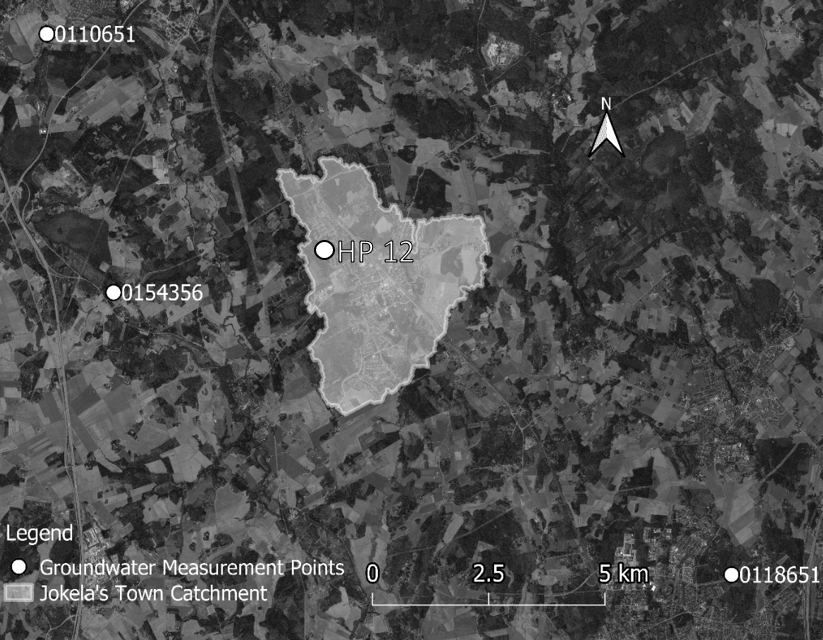
\includegraphics[scale=0.75]{figures/gwmeasurement_points.png}
	\caption{Location of Observation Wells around Jokela's catchment}
	\label{fig:gwmeasurementpoints}
\end{figure}

Data of measurements from 2004 to 2016 of station 0118651 -located southeast from Jokela- were collected. Years with less than six months recorded were left out: 2007; 2008; and 2017. All the eleven years records showed an elevation on the groundwater table from March to May.

Only yearly measurements were available for the station 0154356 located around 5km west from Jokela. The records are from different months, mostly during spring and summer. Therefore, assessment of monthly variation for the same year was not possible. However, the available data suggests slightly higher water table levels on average from January to June for the period of 1999-2017.

Only Station 0118651 and HP 12 had measurements from 2018. This year was relevant to compare with flow measurements available in the sewer network (see section \ref{flowdata}). According to the measurements of these two stations, the water table elevation was higher in the first five months of the year (Jan-May) with increase period from February to May and decrease from May to December 2018.
Monthly mean of measured groundwater table from all SYKE's station as well as monthly measurements of 2018 from stations 0118651 and HP 12 were plotted in figure \ref{fig:gwmeasurements}.

\begin{figure}[h]
    \centering
	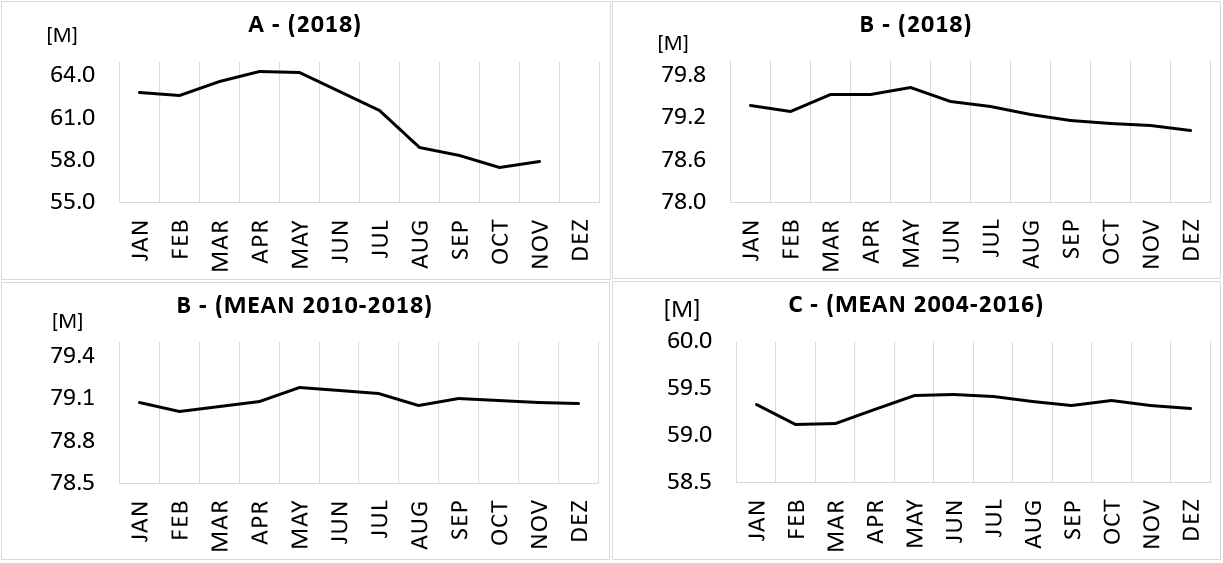
\includegraphics[scale=0.6]{figures/gwmeasurements.png}
	\caption{Groundwater table measurements. Two upper plots are measurements from 2018 only whereas the other two are monthly mean values of the period informed.  (A = H12, B = 0110651, C = 0118651). Data from Tuusulan Vesihuolto and \citet{sykedata}}
	\label{fig:gwmeasurements}
\end{figure}

 
By comparing the two plots of figure \ref{fig:rdiixdwf} and figure \ref{fig:gwmeasurements}, it is possible to observe that a correlation between higher groundwater table and infiltration amount for the first five months into the sanitary sewer of 2018 exists. The estimated amount of RDII peaks on April as the groundwater table elevation measured by the closest observation well to the Jokela's \ac{SSN} (H 12).

As the other data assessed in this study, care should be taken when extrapolating the behavior of the measurements to different years. Groundwater elevation also varies on year by year basis and the same behavior is not always observed. However, the plots of figure \ref{fig:gwmeasurements} presenting the mean values for two different observation wells suggests that an increase of the groundwater table occurs from February to May on average from 2004-2018. 
    


For simplicity, it was assumed that all subcatchments modeled in SWMM share an aquifer with the same characteristics, but with different groundwater infiltration capacity. Therefore, the estimation of parameters is divided here in two parts: 1. Aquifer Parameters and 2. Groundwater Flow Parameters. The choice for different groundwater infiltration parameters for each of the subcatchments was made as an attempt to investigate differences in groundwater infiltration quantity during calibration process. In other words, a higher rate of groundwater infiltration ($f_G$) in one of the subcatchments could suggest that there are more defects (i.e. pipe cracks) to its network and, therefore, could be candidate for further rehabilitation analysis.

\begin{figure}[h]
    \centering
	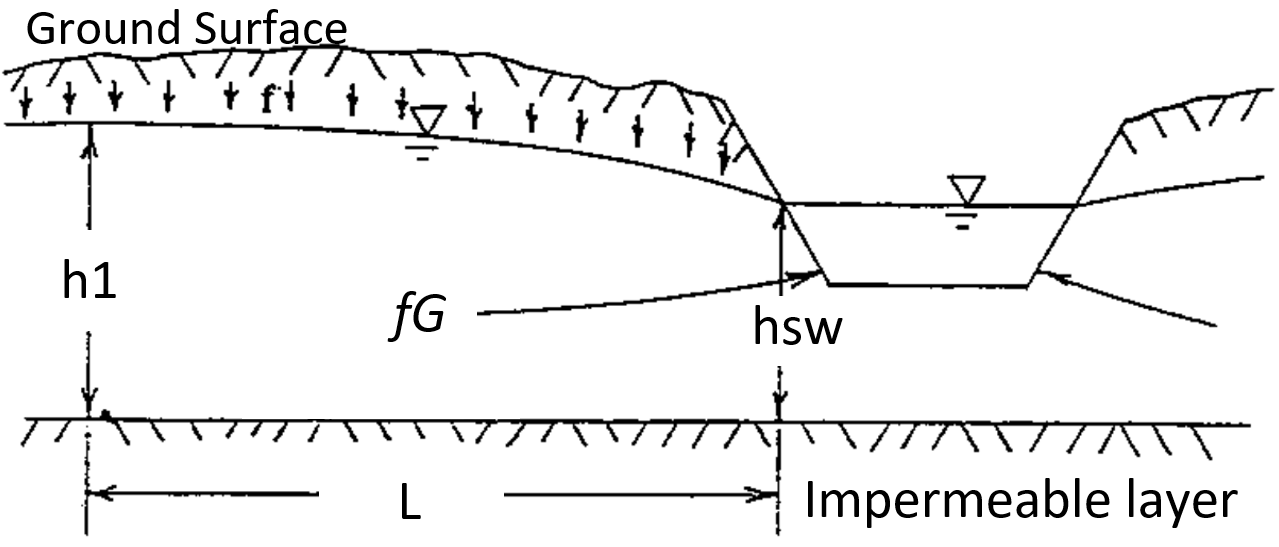
\includegraphics[scale=0.4]{figures/dfscheme.png}
	\caption{Dupuit-Forcheimer lateral seepage to adjacent channel. Modified from} %\cite{bouwer1978}
	\label{fig:dfscheme}
\end{figure}

Dupuit-Forcheimer Lateral Seepage equation (\ref{eqn:dfeq}) was chosen to calculate $f_G$. There was no indication that this choice was the best for the study area. The reasons why Dupuit-Forcheimer was chosen over the three examples described in in SWMM's hydrology reference manual \cite{Rossman2016} were:  1. Unlikely the linear reservoir method, all parameters of the equation could be estimated based on topographical data before calibration process; 2. Simpler than hooghoudt's method since the groundwater infiltration flow is evaluated only at one node. Dupuit-Forcheimer seepage scheme is depicted in figure \ref{fig:dfscheme}.



\begin{equation}
\label{eqn:dfeq}
f_G = A_1 \cdot d^2_L - A3 \cdot d_L\cdot h_{sw}
\end{equation}
where: \\
\indent $f_G$ = Flux from saturated zone to receiving node [m/s] \\
\indent $A1$ = - $A3$ = $2K_s \cdot L^{-2}$ [s m]\textsuperscript{-1}\\
\indent $K_s$ = $f_\infty$ = Saturated hydraulic conductivity [m/s]\\
\indent $L$ = Distance between h1 and $h_{sw}$ [m]\\
\indent $d_L$ = Saturated zone elevation [m]\\
\indent $h_{sw}$ =  Elevation of water inside the receiving node with same reference as the other elevations [m]\\


it was assumed that the water table elevation distribution is similar to the surface elevation spatial distribution to estimate $L$ parameter. This is a rough estimate since there is no indication that the water table elevation follows the surface elevation in the study area. For this, the location of highest surface elevation point per each subcatchment was found using available DEM data and Qgis raster calculator. This point was assumed to be h1 and its distribution is showed in figure \ref{fig:h1position}. The chosen equation is valid only for flows entering the receiving node. Thus, flow occurs only when $d_L$ > $h_{sw}$.

\begin{figure}[h]
    \centering
	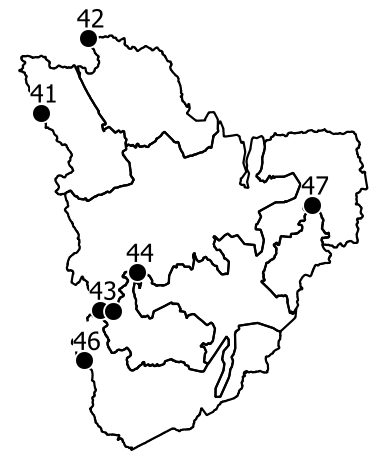
\includegraphics[scale=0.6]{figures/h2position.png}
	\caption{Position of h2 for each subcatchment}
	\label{fig:h1position}
\end{figure}


The distance between these two points were measured and assigned to $L$ for each subcatchment groundwater component. The saturated hydraulic conductivity ($K_s$) was assumed to be constant for all subcatchments and its value was estimated in section \ref{infiltrationcs}. $d_L$ is computed every time step of the simulation, but its initial value ($d_{L0}$) is required and it was set as the bottom elevation of each receiving node ($h_B$) as depicted in table \ref{tbl:gwparamest}. The aquifer bottom elevation used as reference for all the other elevations was also set as $h_B$ since no information of the impermeable zone was assessed. $h_{sw}$ value is obtained from hydraulic model flow routing as the wastewater depth plus $h_B$.

The aquifer parameters were estimated from soil properties data tables available in the literature (\cite{Rawls1983},\cite{Rossman2016}) s done for infiltration parameter estimation also using equation \ref{eqn:infilaverage} to average the values from each subcatchment to the entire catchment area. The parameters and respective estimated values are as follows:

\begin{itemize}
    \item porosity = 0.41 [m³/m³]
    \item field capacity = 0.27[m³/m³]
    \item wilting point = 0.18 [m³/m³]
    \item Tension slope = 15
    \item hydraulic conductivity slope = 48.6
    \item Fraction of evaporation = 0.35 [fraction] 
    \item Lower Evap. Depth = 5 [m]
    \item Lower GW Loss Rate = 1 [m/s]
    \item Initial Unsat. Zone Moisture = 0.27 [fraction]
\end{itemize}

As mentioned on section \ref{jokelatown}, there are streams crossing the delineated catchment area not included in the model. This can be observed when checking the two-aquifer model water budget since interaction between aquifer and surface water (rivers and streams) is not modeled omitting a probably considerable baseflow loss. This loss is represented, in this study, by the seepage to deeper aquifers ($f_L$). The constant rate of seepage is a user-supplied parameter and was used as one of the calibration parameters to simulate long term groundwater table elevation. 

\begin{table}[h]
\caption{Groundwater Flow parameter estimation}
\label{tbl:gwparamest}
\centering
\begin{tabular}{cccc}
\toprule
\multicolumn{1}{l}{\textbf{Subcatchment}} & \textbf{h\textsubscript{B} {[}m{]}} & \textbf{L {[}m{]}} & \textbf{A1  {[}s.m{]}\textsuperscript{-1}} \\ \hline
41                                        & 75.25                 & 1108               & 4.3E-05                                    \\
42                                        & 66.17                 & 2026               & 1.3E-05                                    \\
43                                        & 60.04                 & 2040               & 1.3E-05                                    \\
44                                        & 62.22                 & 1397               & 2.7E-05                                    \\
45                                        & 58.09                 & 1324               & 3.0E-05                                    \\
46                                        & 52.2                  & 1797               & 1.6E-05                                    \\
47                                        & 64.2                  & 1319               & 3.0E-05                                   \\
\bottomrule
\end{tabular}
\end{table}
 
 
Calibration of $L$ parameter may apply as h1 were located, as expected, at the borders of the subcatchments with the rough estimation described above. It is likely that h1 is located further than it is in reality. The calibration should then move towards decreasing the value of $L$. This decrease would result on an increase for $A1$ values resulting on an increase in the groundwater infiltration rate. A flow rate not greater than the observed is expected when using the initial values as suggested in table \ref{tbl:gwparamest} assuming a constant saturated hydraulic conductivity ($K_s$). Therefore, $f_G$ is likely closer to its lower limit range and calibration efforts should focus on increasing $f_G$ by decreasing $L$. 

First simulation was carried with the values presented on table \ref{tbl:gwparamest}. The result of the first simulation of groundwater table ($d_L$) from subcatchment 41 is plotted in figure \ref{fig:gw1stsim}. The variation of the simulated groundwater table did not follow completely the pattern observed from well HP 12 even though both simulated and measured data are from the same delineated area (subcatchment 41). There is an overall increase on the simulation from Jan to May. However, a decrease on $d_L$ from February to March was simulated, but not observed.

It is also important to note that the average elevation of the bottom of the junctions in Jokela's \ac{SSN} is higher than the groundwater table measured (figure \ref{fig:gwmeasurements} suggesting that the groundwater infiltration into the \ac{SSN} is not caused by the water table elevation per se, but by the increase in the soil moisture during aquifer recharge periods (such as snowmelt periods). This is the reason the initial $d_L$ elevations were set as the bottom elevation of the network's receiving node instead of the measured values. The groundwater elevation results from the model simulations is rather a representation of the increase in soil moisture caused by infiltration than the actual groundwater table levels of the aquifer in the sewershed. 

\begin{figure}[h]
    \centering
	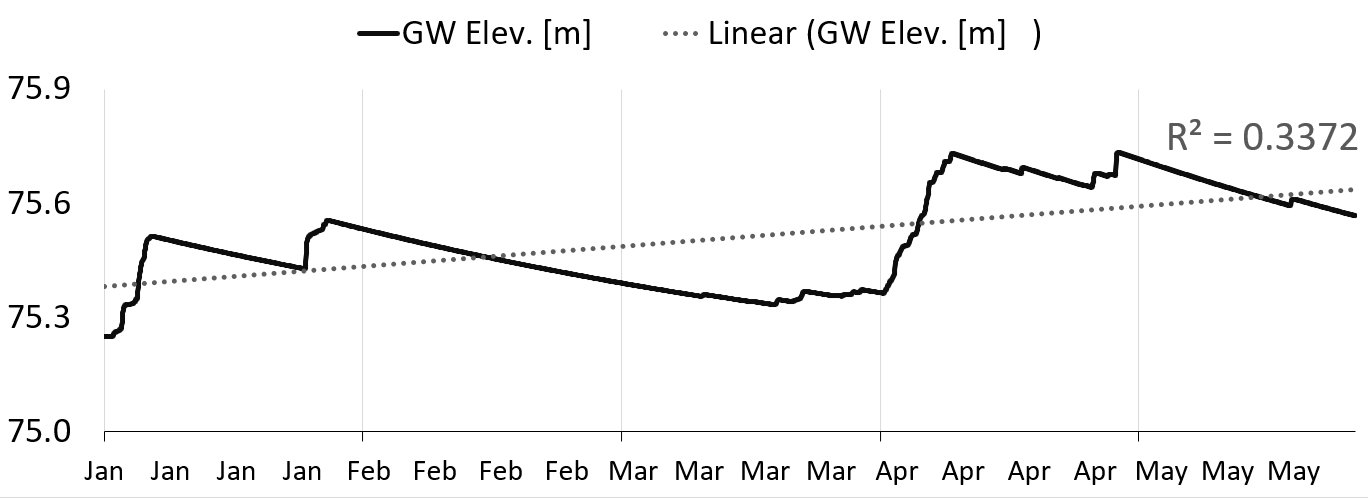
\includegraphics[scale=0.5]{figures/gw1stsimulation_gwlevel.png}
	\caption{Groundwater table first simulation from January to May of 2018}
	\label{fig:h1position}
\end{figure}



% \section{Jokela Sanitary Sewer Model}
% tell about the two different models
% mention more details on the hydraulic model and reference section above



% \subsection{Physically-Based: SWMM Modules}

% Show picture of the model, tell about all the modules used and a table with all parameters estimated

% \begin{figure}[ht]
%     \centering
% 	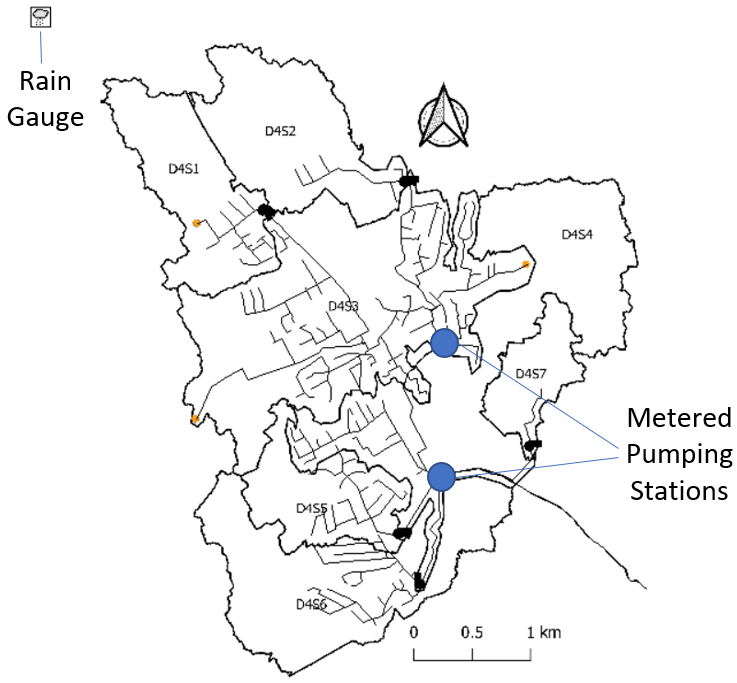
\includegraphics[scale=0.65]{figures/swmm_model.png}
% 	\caption{Groundwater table first simulation from January to May of 2018}
% 	\label{fig:h1position}
% \end{figure}

\subsection{Synthetic Unit Hydrograph: RTK}

Synthetic Unit Hydrographs RTK were added to each of the seven pumping stations as a representation of the hydrological response of each of the delineated subcatchments as illustrated in figure \ref{fig:rtkmodelhydro}. The available parameters to be estimated for each sewershed are in total 15:
\begin{itemize}
    \item $R_{short}, R_{medium}, R_{long}$
    \item $T_{short}, T_{medium}, T_{long}$
    \item $K_{short}, K_{medium}, K_{long}$
    \item $Dmax_{short}, Dmax_{medium}, Dmax_{long}$
    \item $Drec_{short}, Drec_{medium}, Drec_{long}$
\end{itemize}


A literature review was carried to find a suitable range for the estimation of parameters, but they may vary greatly according to the type of watershed being studied. As an example, one may expect a different range of parameters between highly urbanized and semi-urban or rural areas.
As stated by \citet{Vallabhaneni2007} R-values are proportional to the sewershed delineated area. As a hypothetical exercise one can image the differences in the are of the two delineation methods depicted in figure \ref{fig:d1d3} with D3 having a larger area. The fraction of rain falling over the D3 area that finds its way into the sewer system is smaller than the fraction of D1. As the R-values are calibrated to be further multiplied by the sewershed area resulting the desired volume entering the pipe network.
Precipitation input data is another factor influencing the estimation of R-values. In case precipitation measurements used for calibration of R-values fails to capture the realistic volume falling over the sewershed, estimated R-values will also represent erroneous fractions of the precipitation entering the sanitary sewer network. 
Although distinct precipitation measurements lead to different R-values, rain gauges and radar in some cases do capture similar rainfall pattern as concluded by (\citet{wride2004}). Therefore, both rain gauge and radar may yield similar T and K estimated values.
In summary, R-values are influenced by sewershed area, precipitation input, network and catchment’s characteristics 
%//include network characteristics that influences R-values such as aging, defects, etc.  
\citet{Barden2015} applied RDII UH for continuous simulation of a catchment with residential dominant land use and obtained a range of 4 to 26\% for R-values for 14 months recorded period. The study obtained the best results when applying seasonal RTK-values with monthly IA parameters and well performing model for moderate and large storms with seasonal RTK and IA parameters. 
\citet{Vallabhaneni2007} proposes a range for RTK parameters in urban sewersheds depicted in table \ref{tbl:rtkrange}. This range was added as limits for the DDS optimization algorithm.

\begin{table}[h]
\caption{Range of RTK parameters by \citet{Vallabhaneni2007}}
\label{tbl:rtkrange}
\centering
\begin{tabular}{ccc}
\toprule
\textbf{Curve} & \textbf{T {[}h{]}} & \textbf{K} \\ \hline
Short-Term     & 0.5 - 2            & 1 - 2      \\
Medium-Term    & 3 - 5              & 2 - 3      \\
Long-Term      & 5 - 10             & 3 - 7   \\
\bottomrule
\end{tabular}
\end{table}


% We can use T and K as proposed by Vallabhaneni et al. and R based on first calibration. (ex. Manually calibrate three Sewersheds upstream tehtaantie ps and find the maximum Total R value. Consider it was R-20%.   Divide 20% proportionally to the sewershed areas. Ex. S1 Rmax1 = 10%, S2 Rmax2 = 5%, S3 Rmax3 = 5%. Do a similar process to find Rmin values. From that, define the range. Give these limits to the optimization algorithm.
% Do similar for the sewersheds upstream Jokela Ps. (Jokela Flow – Tehtaantie Flow). 

% Separate the calibration of each sewershed to leave room for further analysis when flow meters will be installed to each storage unit.
% The process of finding the R-max and R-min during the calibration process could also be automatized. What was the R-max assigned to an event for the period from May to November? What was the R-min? If the calibration process will be repeated monthly, by the end of the period (November) the 6 months data with each R-value calibrated for each event would be gathered and summed up with the previous years. R-min and R-max could be then fetched from this database and stored for the next calibrations.


\begin{figure}[ht]
    \centering
	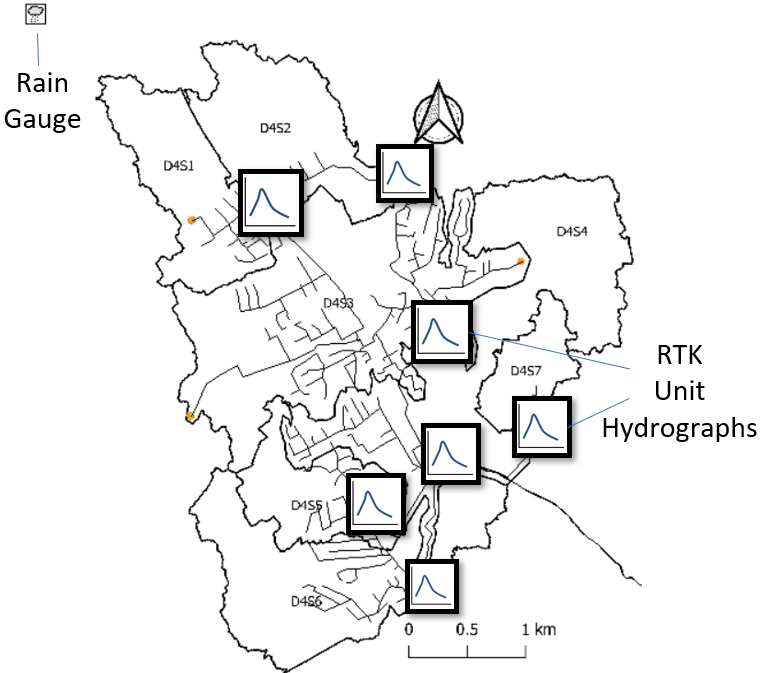
\includegraphics[scale=0.45]{figures/swmm_rtk_model.png}
	\caption{Representation of Jokela's Hydrological Model using RTK UH method}
	\label{fig:rtkmodelhydro}
\end{figure}

%===============================================================
% Simulations
%===============================================================

% \section{Simulations}

% talk about the simulations done and the method for comparing the results (nash suttclife or RMSE, etc). 

\section{Calibration}

\subsection{Calibration of physically based model}
[to do]\\
- include the table with the manually calibrated values for all parameters\\
- Maybe include the results of optimization algorithm results (if time allows) .\\


First calibrations were carried for long-term period of the first five months of 2018 (from Jan to May). The groundwater flow into the \ac{SSN} was lower as expected once the flow parameters were set to the minimum proposed range. Parameter $A1$ value was then increased to approximated one order of magnitude higher. Figure \ref{fig:result_pb_dupuit} depicts the results with the increased values of $A1$. 


\begin{figure}[h]
    \centering
	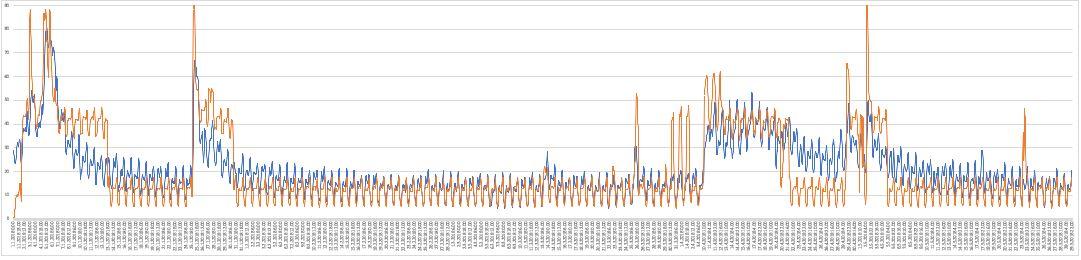
\includegraphics[scale=0.65]{figures/result_pb_depuit_forcheimer.JPG}
	\caption{Long-term simulation of winter period evaluated at Jokela Pumping station using Dupuit-Forcheimer and unidirectional flow condition. Simulated = Orange, Observed = Blue}
	\label{fig:result_pb_dupuit}
\end{figure}



The time of flow increase was successfully achieved. The snowmelt routine successfully utilizes the weather input parameters provides water that infiltrates recharging the aquifer and increasing the flow into the \ac{SSN}. Sharp peaks were also simulated successfully by the runoff module in the same period as the observed values. However, the flow magnitudes were still over estimated and the groundwater flow was abruptly interrupted by SWMM routine that sets the GWI flow to zero once the groundwater table drops below the level of the water in the receiving node. SWMM uses this routine whenever $A3$ value parameter is set to different than zero.

The runoff block parameter $\%routed$ was calibrated as described in section \ref{runofflit} to simulate losses caused by non-modeled streams and stormwater sewer network. To avoid sudden drops of groundwater flow, the A3 parameter was set to zero modifying the firstly proposed Dupuit-Forcheimer formula \ref{eqn:dfeq} excluding the second term to equation \ref{eqn:dfeqmod}.

The flow characteristics of the winter period was much better simulated with groundwater infiltration following the pattern of observed data as depicted in figure \ref{fig:result_pb_nondupuit}. Some ajustments to runnoff parameters are still necessary as well as groundwater flow parameters for periods with severe snowmelt.

\begin{equation}
\label{eqn:dfeqmod}
f_G = A_1 \cdot d^2_L
\end{equation}

\begin{figure}[h]
    \centering
	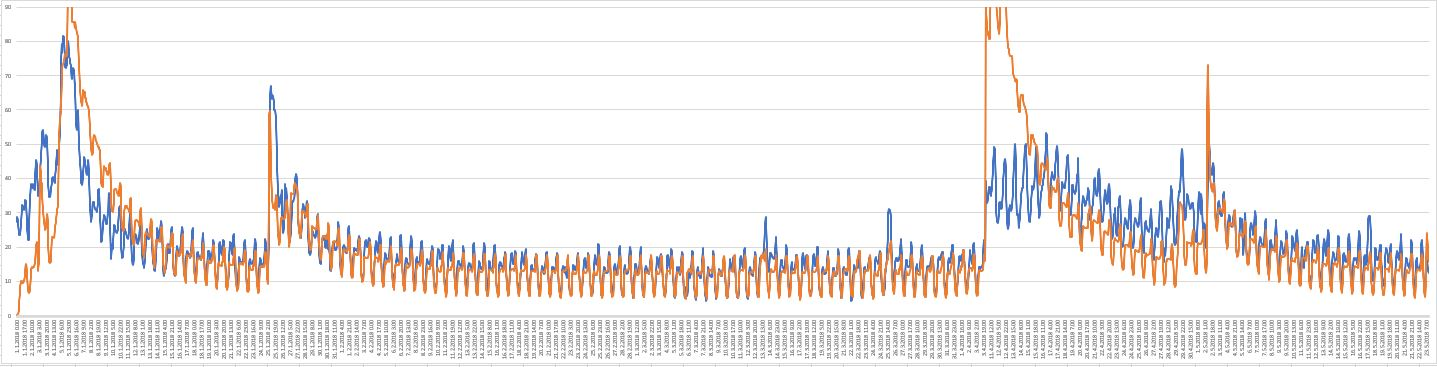
\includegraphics[scale=0.45]{figures/result_pb_non_forcheimer.JPG}
	\caption{Long-term simulation of winter period evaluated at Jokela Pumping station using different GWI equation and unidirectional flow condition. Simulated = Orange, Observed = Blue}
	\label{fig:result_pb_nondupuit}
\end{figure}



\subsection{Calibration of RTK Model}
[to do]\\ \\
- better description of the calibration algorithm used and the search space.\\
- include calibration results of other storms chosen for parameter calibration. Not figures, but maybe a table with nash-sutcliffe/RMSE and errors in peak and volume of the respective storm) .\\

The first storms used to investigate the performance of RTK model with DDS optimization algorithm occurred in 2018 summer from July 1st to July 6th. The reason why this period was chosen is that different storm intensities were recorded causing sharp increase in the sanitary sewer flows as depicted in figure \ref{fig:rain04}. 

\begin{figure}[h]
    \centering
	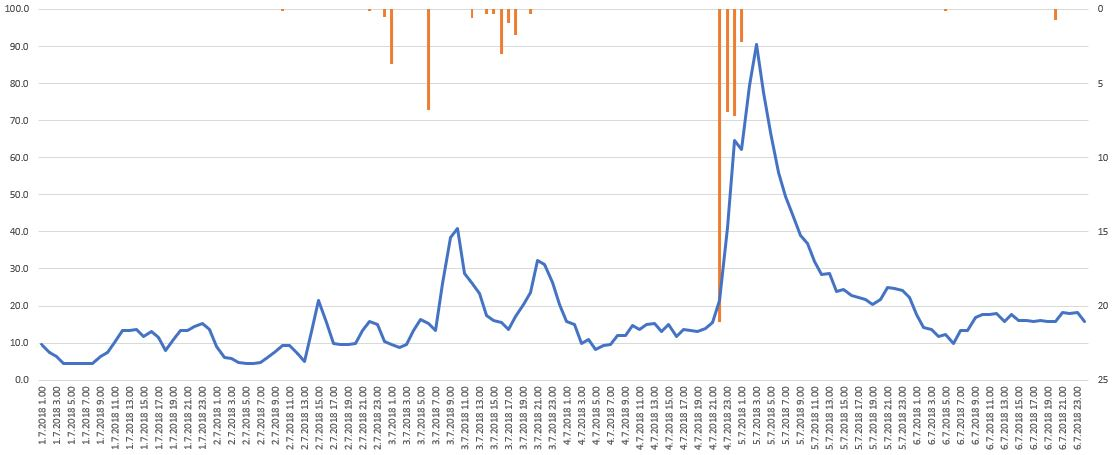
\includegraphics[scale=0.45]{figures/rain04.JPG}
	\caption{Rain 04}
	\label{fig:rain04}
\end{figure}

Figures \ref{fig:calibration06_rain04_100steps}, \ref{fig:calibration05_rain04_300steps}, \ref{fig:calibration09_rain04_600steps}, and \ref{fig:calibration04_rain04_1000steps}, have the plot of simulated versus observed results where DDS optimization algorithm was set to use respectively 100, 300, 600, and 1000 iterations. 

Table \ref{tbl:rtkresults} depicts the results evaluated by nash-sutcliffe and root mean square error coefficients for pumping station 1 and pumping station 2.

\begin{table}[h]
\caption{RTK rain 04 simulation results evaluation. Nash-Sutcliffe = 1 means a perfect model}
\label{tbl:rtkresults}
\centering
\begin{tabular}{ccccc}
\toprule
\textbf{Number of Iterations} & \multicolumn{2}{c}{\textbf{Nash-Sutcliffe}} & \multicolumn{2}{c}{\textbf{RMSE}} \\ \cline{2-5} 
                              & PS1                  & PS2                  & PS1             & PS2             \\ \cline{2-5} 
100                           & 0.82                 & 0.81                 & 6.49            & 4.59            \\
300                           & 0.85                 & 0.85                 & 6.02            & 4.08            \\
600                           & 0.86                 & 0.86                 & 5.68            & 3.98            \\
1000                          & 0.88                 & 0.79                 & 5.39            & 4.75     
\\ \bottomrule
\end{tabular}
\end{table}


\begin{figure}[h]
    \centering
	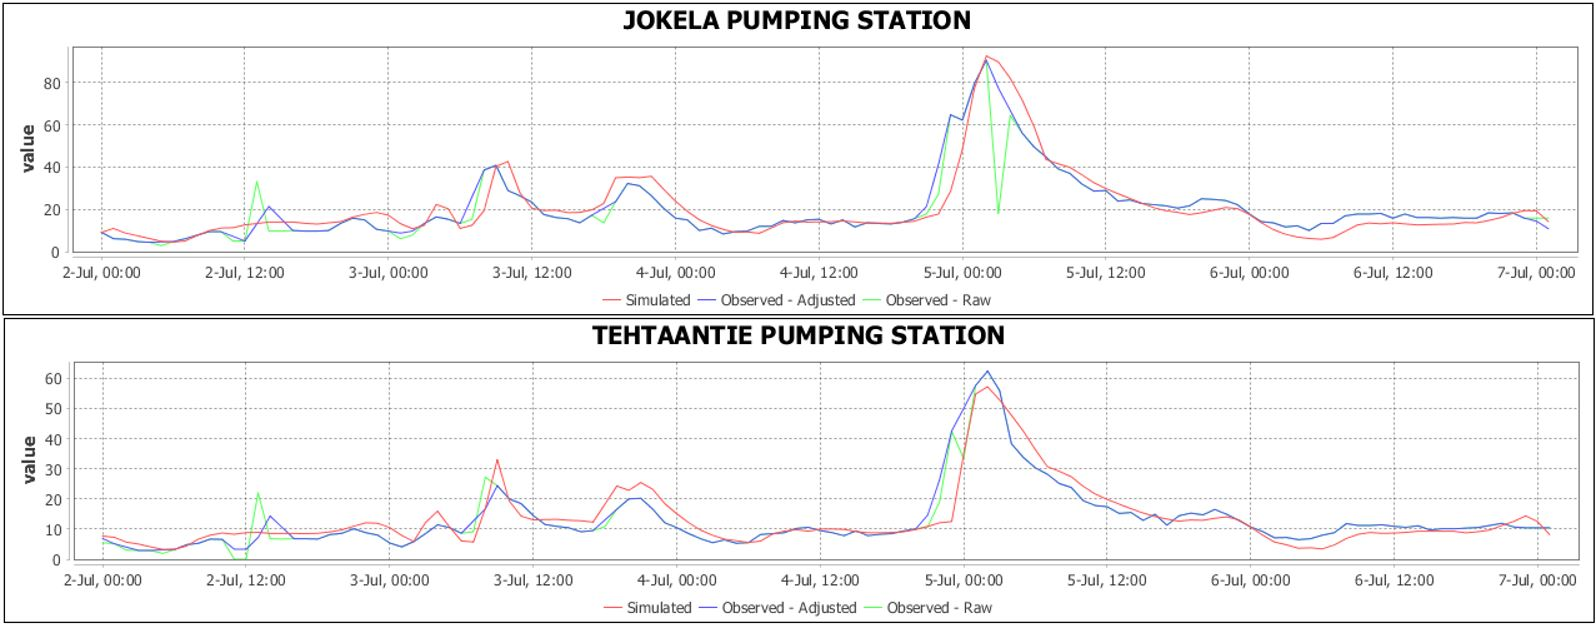
\includegraphics[scale=0.45]{figures/calibration06_rain04_100steps.JPG}
	\caption{Calibration results of RTK parameters using Rain04 and 100 iterations of DDS optimization algorithm}
	\label{fig:calibration06_rain04_100steps}
\end{figure}

\begin{figure}[h]
    \centering
	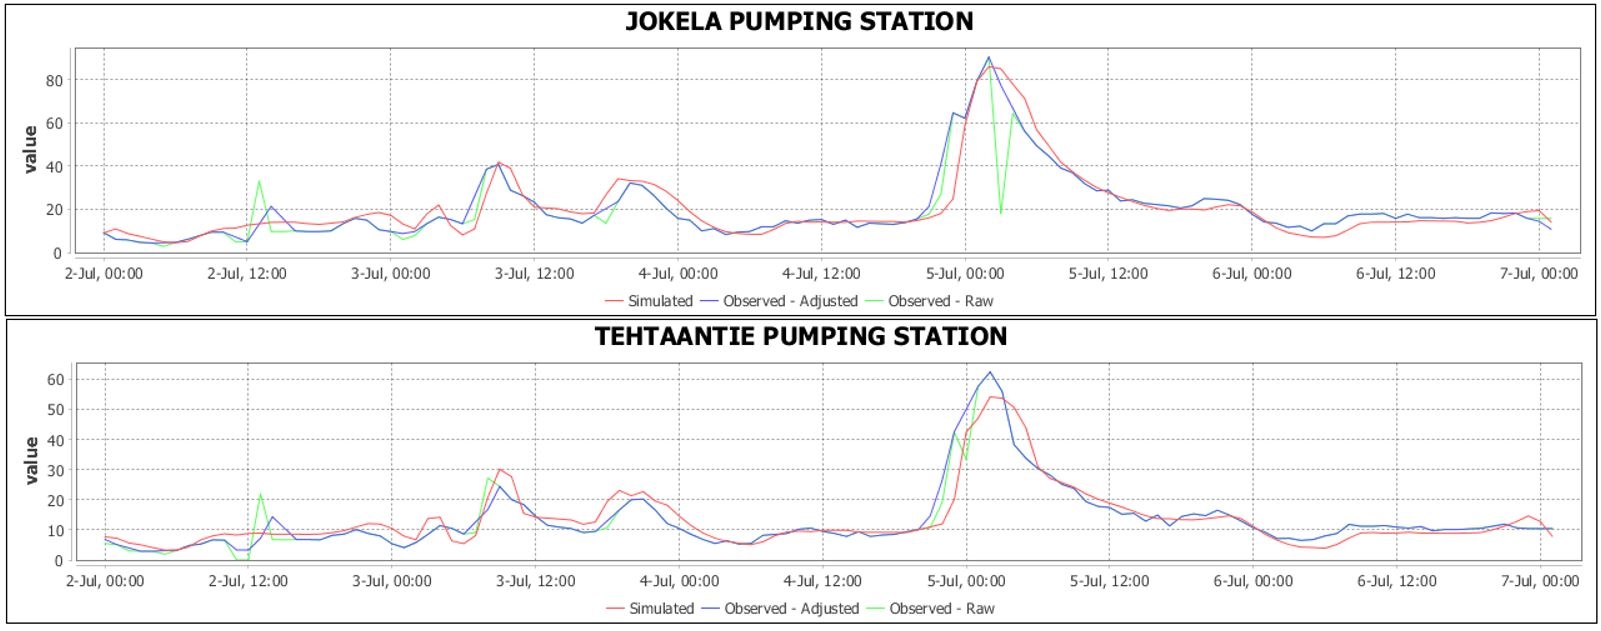
\includegraphics[scale=0.45]{figures/calibration05_rain04_300steps.JPG}
	\caption{Calibration results of RTK parameters using Rain04 and 300 iterations of DDS optimization algorithm}
	\label{fig:calibration05_rain04_300steps}
\end{figure}

\begin{figure}[h]
    \centering
	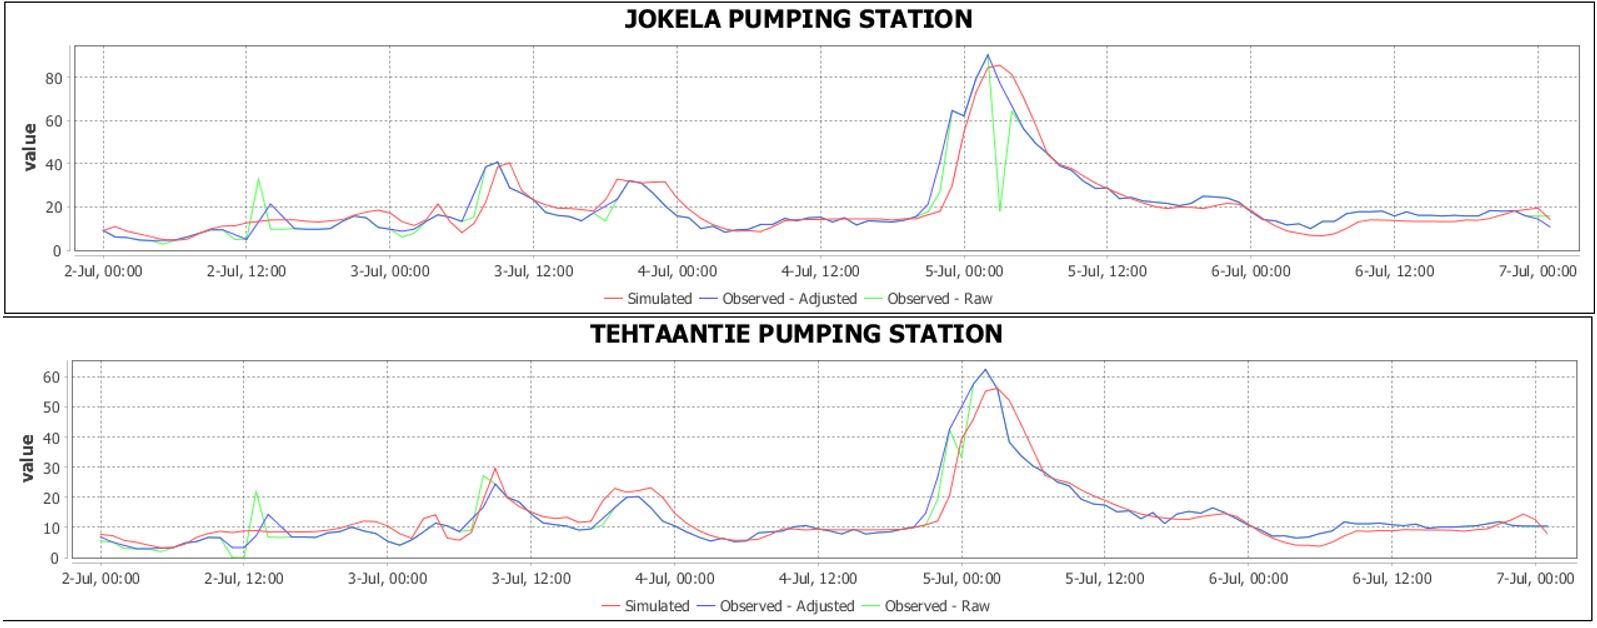
\includegraphics[scale=0.45]{figures/calibration09_rain04_600steps.JPG}
	\caption{Calibration results of RTK parameters using Rain04 and 600 iterations of DDS optimization algorithm}
	\label{fig:calibration09_rain04_600steps}
\end{figure}

\begin{figure}[hb]
    \centering
	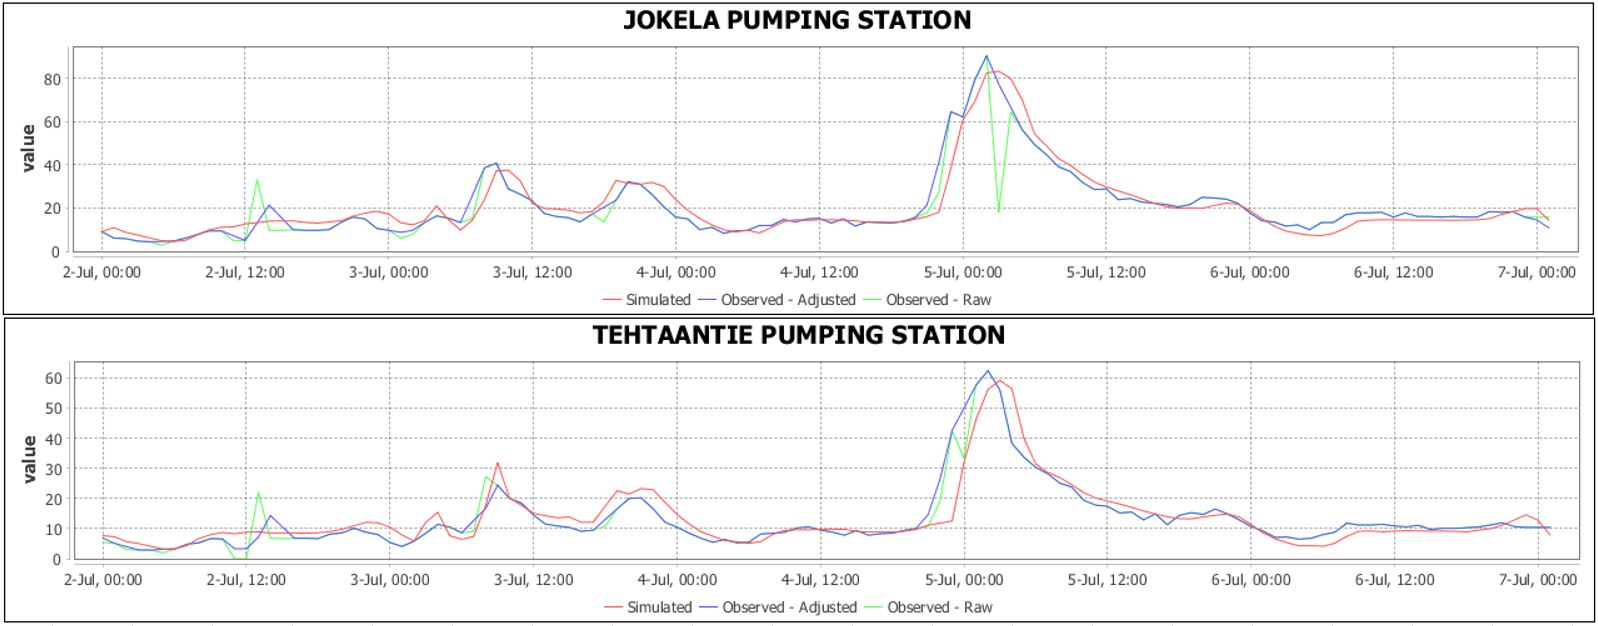
\includegraphics[scale=0.45]{figures/calibration04_rain04_1000steps.JPG}
	\caption{Calibration results of RTK parameters using Rain04 and 1000 iterations of DDS optimization algorithm}
	\label{fig:calibration04_rain04_1000steps}
\end{figure}


\section{Validation}

\section{Validation with historical Meteorological Data}
[to do]\\

\section{Validation with historical Weather Forecast Data}
[to do]\\

- flow data of 2019 that will be used for the validation using weather forecast received today (15.07.19).\\